\chapter{Resultados y validación}

\section{Introducción}
La validación es una etapa crítica en el proceso de desarrollo de cualquier proyecto, especialmente en un proyecto de la magnitud y complejidad del convertidor diseñado. La validación se encarga de verificar que todos los componentes y subsistemas del convertidor funcionen correctamente y cumplan con los requisitos y especificaciones establecidos previamente.

Dada la naturaleza multifacética del convertidor, que abarca desde aspectos eléctricos y electrónicos hasta aspectos de control y \textit{firmware}, es esencial planificar una estrategia de validación exhaustiva y efectiva. En este sentido, se ha adoptado un enfoque metodológico basado en el modelo en V, que permite validar los subsistemas desde los más específicos hasta los más generales, siguiendo un flujo lógico y sistemático. 

En este capítulo se desarrolla la parte derecha de la 'V', diseñando y ejecutando las pruebas a varios niveles. La estrategia de validación comenzará validando el \textit{hardware}, desde los componentes individuales hasta las placas enteras, y continuará con una etapa de integración en la que se desarrolla el \textit{firmware}. Cada bloque tiene sus propios desafíos y requisitos específicos, pero todos contribuyen al objetivo final de asegurar el funcionamiento correcto y robusto del convertidor. Las diferentes partes de la validación que se han encarado de formas también diferentes, atendiendo a las circunstancias y priorizando las buenas prácticas y la identificación de problemas a los resultados exitosos.

\section{Validación de \textit{hardware}}

La parte más crítica en la validación del convertidor es la de \textit{hardware} puesto que cada iteración cuesta tiempo y dinero. Por ello, son las pruebas de \textit{hardware} las que se diseñan y ejecutan más meticulosamente. En particular, se prestó especial atención a la placa de potencia, puesto que es el diseño más complicado de los dos.

Inicialmente, se elaboraron hojas de cálculo detalladas para cada uno de los ensayos, abarcando desde la inspección visual y pruebas de subcircuitos, hasta la evaluación de sistemas algo más complejos. Sin embargo, a medida que avanzaba el proceso de validación y se integraban los subcircuitos unos con otros, se hizo evidente que era necesario un enfoque más dinámico y adaptativo. Esto se debió a que los problemas encontrados y las soluciones implementadas requerían una validación continua y menos estructurada, lo que permitía realizar ajustes y mejoras tiempo real. Sin embargo, no por ello se dejaron de documentar los ensayos, si no que se registraron de formas menos profesionales.


\subsection{Pre-inspección de la placa de potencia}
Antes de realizar cualquier prueba funcional, se llevó a cabo una inspección visual exhaustiva de la PCB de potencia para identificar cualquier defecto físico o de manufactura. Esta inspección incluyó la verificación del acabado superficial, la serigrafía, el grosor del cobre en las capas y las dimensiones de la placa. En la primera iteración se encontraron algunos problemas menores, como una serigrafía invertida en los conectores del bus de continua, pero no afectaron las pruebas iniciales.

Se validó el grosor de cobre en las vías para aportar confianza a la hora de montar los componentes \textit{press-fit}. Para ello, se extrajo una sección de la PCB que cortaba transversalmente una vía y se pulió. Posteriormente, se tomó una fotografía con un microscopio y se hicieron medidas digitales.

\begin{figure}[H]
	\centering
	\includegraphics[width=0.7\linewidth]{fig/copperVia1}
	\caption{Extracción de una muestra de la PCB.}
\end{figure}


\begin{figure}[H]
	\centering
	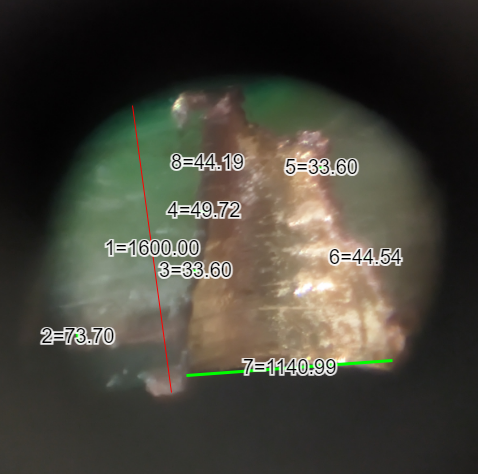
\includegraphics[width=0.7\linewidth]{fig/copperVia}
	\caption{Micrografía de una vía de la placa de potencia. Se pueden apreciar el grosor de cobre de las capas y de la vía.}
\end{figure}

Se pudo comprobar que el grosor de las capas era correcto (70 \unit{\micro\meter}), y que el de las vías estaba dentro de la tolerancia establecida (de 25 a 50 \unit{\micro\meter}).

\subsection{Primer contacto con la placa de potencia}

Durante la primera interacción con la placa de potencia, se realizaron diversas pruebas para validar el funcionamiento de los distintos componentes y subcircuitos de forma aislada. Principalmente se busca validar una funcionalidad básica de cada uno de forma separada, de manera que si se encuentran problemas de integración se sepa que son de integración y no de los componentes o circuitos individuales. Se ordenaron estas pruebas de "dentro hacia afuera", empezando por el circuito de \textit{driving} y acabando con la interacción externa del mismo. También se validó la adquisición de variables analógicas y se probó la funcionalidad básica del circuito de descarga.


\subsubsection{Alimentación del \textit{gate driver}}

Para validar la alimentación del \textit{gate driver} se separó en una verificación del LDO para la tensión negativa por separado, y en otra para validar el DC-DC.

En primer lugar se pobló únicamente el propio LDO con los componentes necesarios para su funcionamiento. Se anotó el primer error de la placa, que consiste en una equivocación en el mapeado de los pines del esquemático al \textit{footprint}. De todas formas, se realizó un \textit{dead-bugging} para conectar el componente de forma correcta y poder verificar el circuito de forma exitosa.

\begin{figure}[H]
	\centering
	\includegraphics[width=0.7\linewidth]{fig/deadbug}
	\caption{LDO \textit{dead-bugged} y con resina para evitar daños con las siguientes pruebas.}
\end{figure}

\begin{itemize}
	\item \textbf{Valor esperado}: -4 V $\le$ V $\le$ -3,5 V
	\item \textbf{Resultado}: -3,78 V
\end{itemize}


La dificultad de realizar este \textit{rework} fue motivo suficiente para corregir el diseño, pero se esperó a finalizar la mayoría de pruebas básicas antes de pedir placas nuevas.

Después de verificar el funcionamiento del LDO se probaron los DC-DCs aislados. Funcionaron según lo previsto, aunque se notó que se calentaban ligeramente, incluso en vacío (sin carga). Esto se debe a su curva de rendimiento, que con cargas bajas es muy poca. Además se anotaron variaciones en las tensiones de salida, pero resultó que eran función de la carga, y está explicado en la hoja de datos.

\begin{figure}[H]
	\centering
	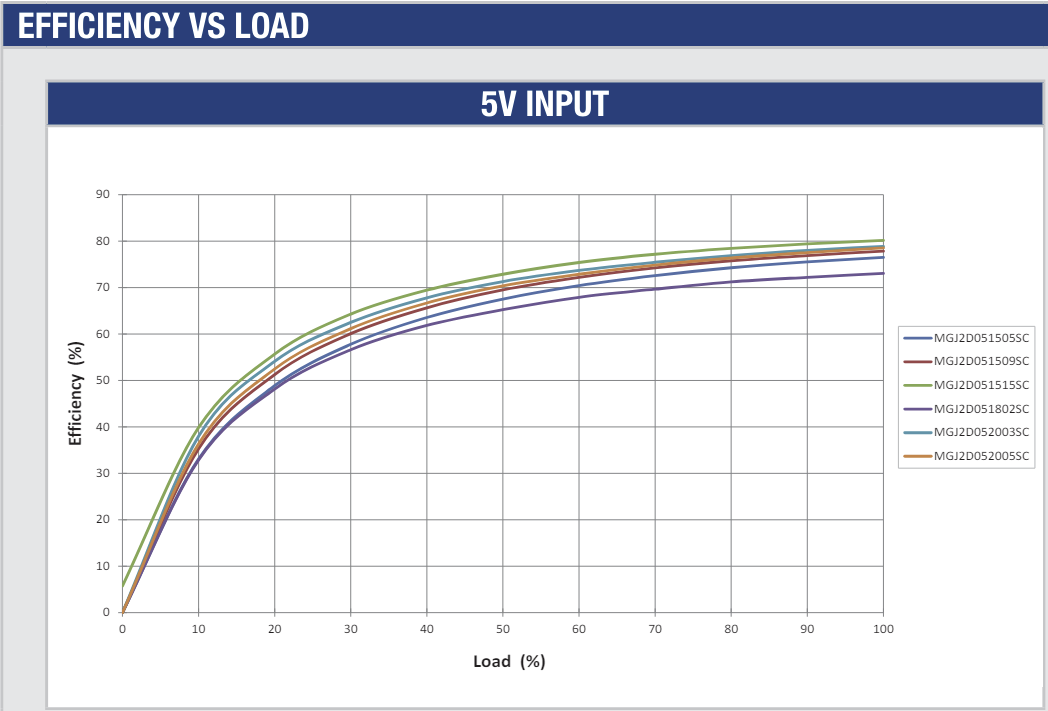
\includegraphics[width=0.7\linewidth]{fig/DCDC-eff}
	\caption{Curva de rendimiento del DC-DC aislado \cite{MurataDCDC}.}
\end{figure}

\begin{figure}[H]
	\centering
	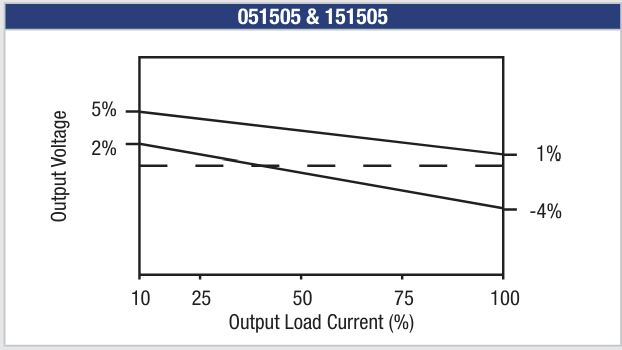
\includegraphics[width=0.7\linewidth]{fig/DCDC-eff1}
	\caption{Variación de la tensión de salida en función de la carga \cite{MurataDCDC}.}
\end{figure}

\begin{itemize}
	\item \textbf{Valor esperado}: 15,5 V $\le$ VDD $\le$ 14,5 V ; -4 V $\le$ VEE $\le$ -3,5 V
	\item \textbf{Resultado}: 15,94 V ; -3,78 V
\end{itemize}

\subsubsection{Funcionalidad del \textit{gate driver}}
Para validar la funcionalidad básica del \textit{gate driver}, se montó un módulo de potencia y los dos \textit{gate drivers} necesarios para controlar los dos MOSFETs.

\begin{itemize}
	\item \textbf{\textit{OK} y \textit{TRIP}}: Se poblaron los componentes necesarios y se alimentó la placa desde el lado de \textit{LV}. Se midieron los nodos \textit{TRIP} y \textit{OK}. Ambas señales tenían un valor de 5 V, confirmando su correcto funcionamiento sin errores. Posteriormente se forzaron fallas en el lado del semiconductor y ambas bajaron a 0 V.
	\item \textbf{MOSFETs apagados en reposo}: Se montaron las resistencias de puerta y se verificó el estado de ambos MOSFETs midiendo la resistencia entre \textit{drain} y \textit{source}. Ambos dispositivos se encontraban en estado \textit{OFF}, confirmando que no se encendían.
	\item \textbf{\textit{ENABLE} no enciende los dispositivos}: Se introdujo una señal de 3,3 V el nodo \textit{ENABLE}, simulando la acción del microcontrolador. De nuevo, ambos dispositivos se encontraban en estado \textit{OFF}, lo cual es el resultado esperado, ya que ambas señales PWM estaban en estado bajo, es decir, consignando que los MOSFETs estuvieran abiertos.
	\item \textbf{Medición de temperatura}: Se verificó la capacidad del \textit{gate driver} de tomar una medida analógica, en concreto, de la NTC interna del semiconductor. Se contrastaron las medidas obtenidas con los cálculos previos, arrojando resultados satisfactorios.
	
	\begin{figure}[H]
		\centering
		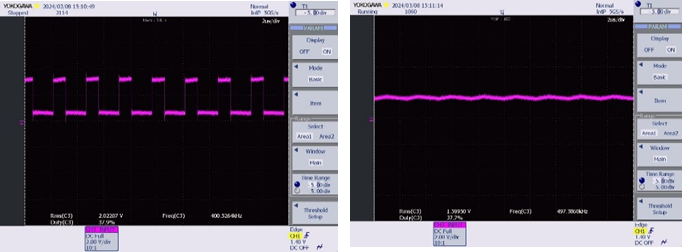
\includegraphics[width=0.7\linewidth]{fig/NTC-driver}
		\caption{Medición de temperatura ambiente. Se puede ver la señal de salida sin filtrar (PWM) y filtrada.}
	\end{figure}
	
\end{itemize}
	
\subsubsection{Sensado de corriente}

Para validar el funcionamiento del sensado de corriente, se realizaron las siguientes pruebas:

\begin{itemize}
	\item \textbf{Standby}: Se esperaba una salida de 2,5 V con un margen de error de $\pm$ 5 mV. La salida medida fue de 2,499 V, lo que se considera dentro del rango aceptable.
	
	\item \textbf{Operación básica}: Se esperaba una salida de 2,5625V para una corriente de +5A y 2,4375V para una corriente de -5 A, con un margen de error de $\pm$ 5 mV. Las mediciones obtenidas fueron de 2.557 V para +5 A y 2,436 V para -5 A, ambas dentro del rango esperado.
\end{itemize}	


\subsubsection{Descarga}

Para verificar la funcionalidad de la descarga, se realizaron las siguientes pruebas:

\begin{itemize}
	\item \textbf{Descarga pasiva}: Se precalculó una descarga de 24 V a 10 V en 35 segundos usando un 20 \% de la capacidad del bus. La medición obtenida fue de 5,5 segundos, debido a que no se tuvo en cuenta el resto de conexiones entre los terminales positivo y negativo. La resistencia aparente entre estos terminales era más baja, principalmente por el divisor de tensión usado para tomar la medida de voltaje del bus. El divisor de voltaje para la adquisición ya es de $6 \cdot 68 \text{ k}\Omega + 4.7 \text{ k}\Omega = 412.7 \text{ k}\Omega$, y está en paralelo con la resistencia de $2 \text{ M}\Omega$, lo que resulta en una resistencia equivalente de 
	$$
	\frac{1}{\frac{1}{2 \text{ M}\Omega} + \frac{1}{412.7 \text{ k}\Omega}} = 342 \text{ k}\Omega,
	$$
	lo que equivale a aproximadamente 6 segundos de descarga. Al agregar cualquier otra resistencia en paralelo, como la de los propios semiconductores u otros componentes, los cálculos coinciden.
	
	\begin{figure}[H]
		\centering
		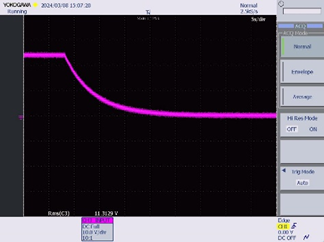
\includegraphics[width=0.7\linewidth]{fig/discharge1}
		\caption{Descarga pasiva a 24 V con 20 \unit{\micro\farad}.}
	\end{figure}
	
	\item \textbf{Control de la descarga}: Se aplicó un voltaje de 20 V en el nodo \textit{SC\_END} y se suministraron 24 V entre \textit{TS+} y \textit{TS-}. Se esperaba que la diferencia de potencial entre \textit{TS+} y \textit{TS-} fuera de 10 V 0,35 segundos después de retirar el voltaje, que coincidió perfectamente con el cálculo previo.
	\begin{figure}[H]
		\centering
		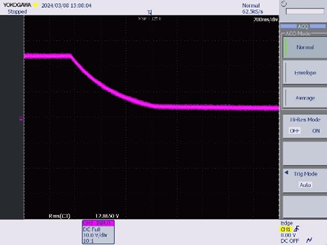
\includegraphics[width=0.7\linewidth]{fig/discharge2}
		\caption{Descarga activa a 24 V con 20 \unit{\micro\farad}. Se puede ver como a 10 V (la tensión del zener) se desactiva la descarga activa.}
	\end{figure}
\end{itemize}
	
	
\subsubsection{Sensado de voltaje}

Para verificar el sensado de voltaje, se llevaron a cabo las siguientes pruebas:

\begin{itemize}
	\item \textbf{Divisor de voltaje}: Se aplicaron 24 V entre \textit{TS+} y \textit{TS-}. Se capturó el voltaje en el divisor de tensión. La tensión esperada era de $0.011388 \cdot 24\text{ V} = 0.2733 \text{ V}$ con un margen de error de $\pm$1 mV. La medición obtenida fue de 0,272 V, dentro del rango aceptable.
	
	\item \textbf{Alimentación aislada}: Se montó el convertidor DCDC501 y se alimentó la placa desde el lado LV para medir el voltaje entre \textit{+5\_TS} y \textit{TS-}. Se esperaba una lectura de 5V con un margen de error de $\pm$0,5 V. Sin embargo, la medición fue de 5,5 V, indicando que se deberá ajustar el divisor de voltaje para el umbral de detección debido a la inexactitud.
	
	\item \textbf{Detección de voltaje}: Se aplicaron 50 V entre \textit{TS+} y \textit{TS-}, y se midió \textit{TSAL\_ON}. Se repitió la prueba con 60 V. Se esperaba que \textit{V\_TSAL} fuera de 677 mV y que \textit{TSAL\_ON} fuera 5 V con 50 V de tensión de bus y 0 V con 60 V. Sin embargo, la medición fue incorrecta, ya que el umbral aproximado para la transición fue de 63 V. Se encontró que la causa podría estar la tolerancia del divisor de resistencia y el hecho de que la salida del convertidor DC-DC era medio voltio superior.

	\item \textbf{Sensado de voltaje}: Se aplicaron 13 V entre \textit{TS+} y \textit{TS-}. Se capturó el valor entre \textit{VDC\_sns+} y \textit{VDC\_sns-}. Se esperaba que la diferencia de potencial fuera de 0,0495 V. La medición obtenida fue de 0,05 V, dentro del rango aceptable.
\end{itemize}

\begin{figure}[H]
	\centering
	\includegraphics[width=0.7\linewidth]{fig/vSensePCB}
	\caption{Circuitos evaluados.}
\end{figure}


\subsubsection{Resumen de errores encontrados y revisión de la PCB}

Se encontraron los siguientes errores durante el proceso de prueba y montaje:

\begin{enumerate}
	\item \textbf{Problema:} El serigrafiado de los conectores de alimentación (+ y -) está invertido. Esto no afecta las pruebas. \\
	\textbf{Solución propuesta:} Nombrar los conectores según corresponda y cambiar los textos del serigrafiado. Pedir nuevas PCBs.
	
	\item \textbf{Problema:} Se conectó accidentalmente el nodo de 5 V de alimentación a \textit{SC\_END} (20 V), lo  que hizo que todos los componentes alimentados a 5 V murieran.\\
	\textbf{Solución propuesta:} Añadir protecciones a la alimentación de 5 V.
	
	\item\textbf{Problema:} El \textit{footprint} del LDO tiene los pines 4 y 5 intercambiados (\textit{-VEE}, \textit{FB}). \\
	\textbf{Solución propuesta:} Montar el LDO verticalmente con conexiones flotantes cruzadas.
\end{enumerate}

Para realizar el resto de pruebas se pidieron nuevas placas de potencia, con las siguientes modificaciones:

\begin{itemize}
	\item Protecciones para la alimentación de 5 V.
	\item Se intercambiaron los pines 4 y 5 en los LDO de los \textit{gate drivers}.
	\item Se intercambiaron \textit{MP+} y \textit{MP-} junto con su serigrafiado.
	\item Se añadieron \textit{testpoints} para la referencia de los sensores de corriente.
	\item Se añadieron \textit{testpoints} para \textit{VDC\_sns+} y \textit{VDC\_sns-}.
	\item Se renombraron los \textit{testpoints} en el esquemático de los \textit{gate drivers} para agilizar las pruebas.
	\item Se añadieron varios textos e indicaciones en el serigrafiado.
\end{itemize}

\subsection{Conmutación de una rama como DC-DC síncrono}

Con todos los subcircuitos validados, el siguiente paso fue analizar la conmutación. Se utilizó una sola rama de las tres, creando una topología de \textit{buck} síncrono. Se ensayó con una carga R-L de 7 $\Omega$ y 1 mH. Lo que se pretende evaluar con estas pruebas es el correcto funcionamiento del circuito de \textit{driving} y el \textit{overshoot} entre \textit{drain} y \textit{source} de los MOSFETs.

\begin{figure}[H]
	
	\centering
	\begin{circuitikz}
		% Upper MOSFETs
		\draw (0,0) node[nigfete,anchor=D,bodydiode] (M1) {};

		
		% Lower MOSFETs
		\draw (0,-2) node[nigfete,anchor=D,bodydiode] (M4) {};

		% Connections
		\draw (M1.S) -- (M4.D);
		
		% Battery
		\draw (M1.D)  |-  ++(-4,0) to[battery, l=$V_{\text{DC}}$] ++(0,-3.5)  |-  (M4.S);
		\draw (M1.D)  |-  ++(-1.5,0) to[capacitor] ++(0,-3.5)  |-  (M4.S);
		
		\draw (M1.S)  |-  ++(2,0) node[right, font=\tiny] {};
		
		\draw (M4.S)  |-  ++(6,0) node[right, font=\tiny] {};
		% Inductor and resistor connected to cable A
		\draw (M1.S) ++(2,0) to[L, l=$L$] ++(2,0);
		\draw (M1.S) ++(4,0) to[R, l=$R$] ++(2,0);
		
		\draw (6,-1.55)  |-  ++(0,-2) node[right, font=\tiny] {};
	\end{circuitikz}
	\caption{Topología de \textit{buck} síncrono.}
	
\end{figure}
	

\begin{figure}[H]
	\centering
	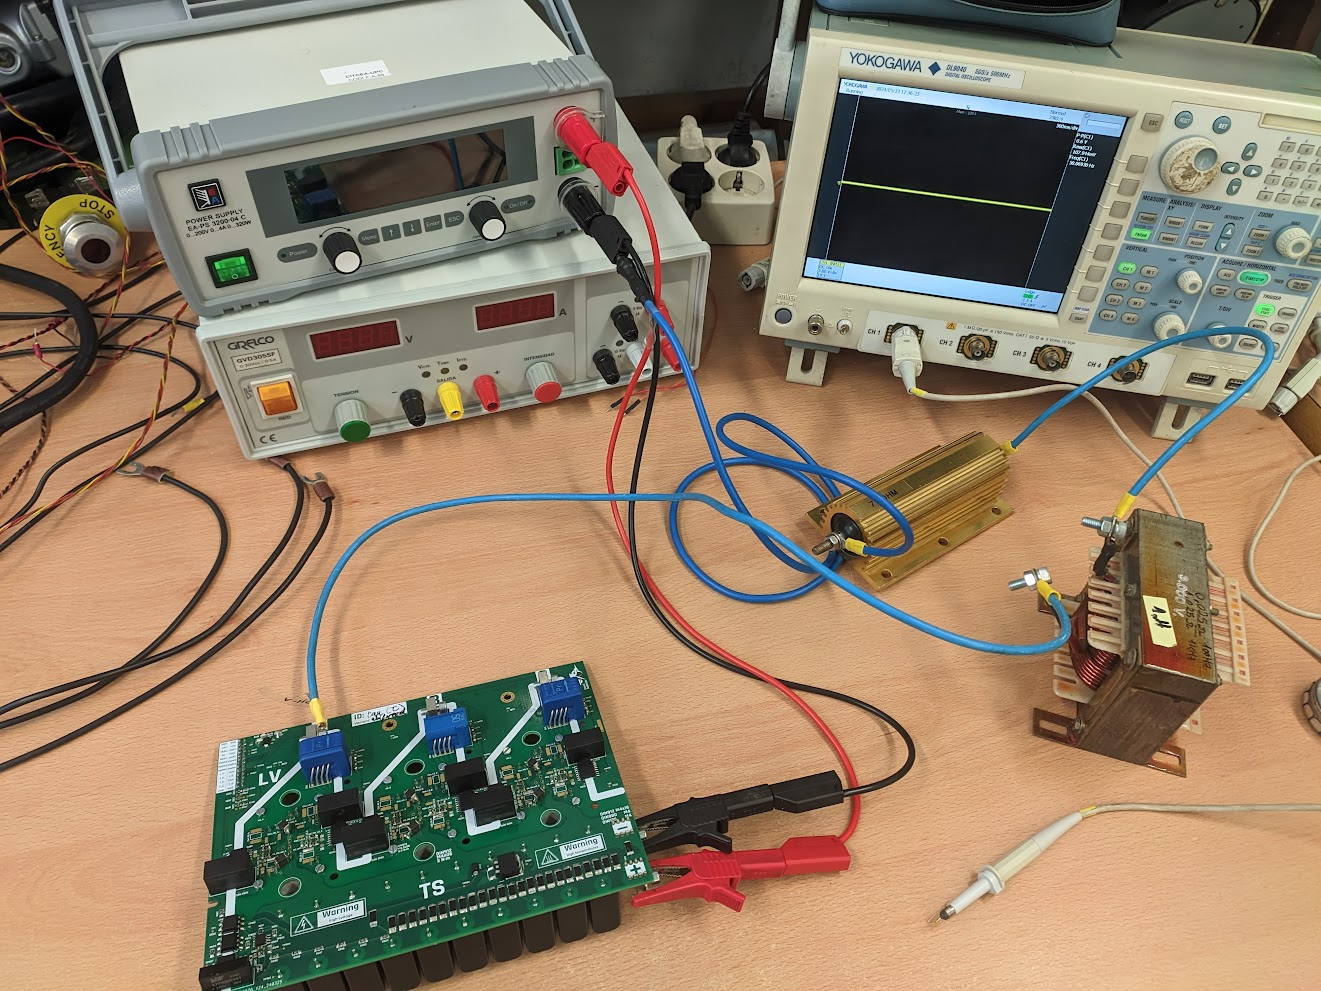
\includegraphics[width=0.7\linewidth]{fig/RL_setup}
	\caption{Carga R-L, fuente de alimentación y osciloscopio.}
\end{figure}


Se conectó la placa de potencia con una placa de evaluación ya que en este punto todavía no se había fabricado la placa de control. De esta manera, se generó una pareja de señales PWM complementarias a 50 kHz y 50 \% de ciclo de trabajo con 150 ns de tiempo muerto. 
	
\begin{figure}[H]
	\centering
	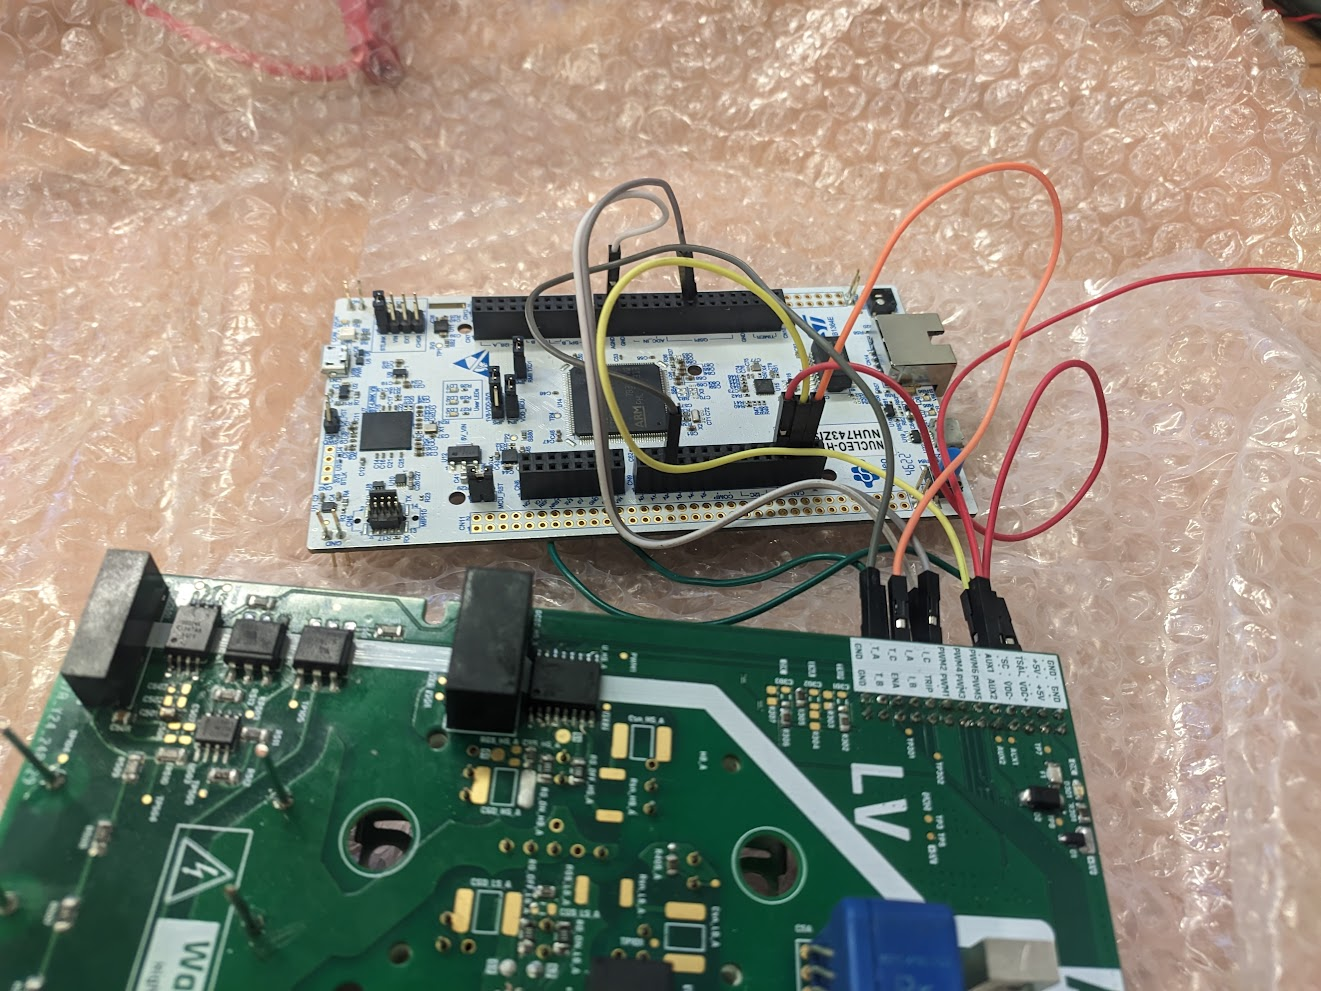
\includegraphics[width=0.7\linewidth]{fig/nucleoHalfBridge}
	\caption{Placa de evaluación Nucleo conectada a la placa de potencia.}
\end{figure}
Usando una fuente de tensión regulable, se pudo controlar la tensión de entrada, y dado que se fija el ciclo de trabajo al 50 \%, y que la carga es fija, se pudo variar la tensión de salida modificando la tensión de entrada. Conectando y desconectando la carga, se pudo probar la conmutación tanto en vacío como con algo de corriente.


En primer lugar, sin tensión en el bus de continua, se verificó que tanto las señales PWM entrantes a los \textit{gate drivers} como las señales en la puerta de los transistores eran adecuadas en cuanto a niveles de tensión, frecuencia y polaridad.

	
\begin{figure}[H]
	\centering
	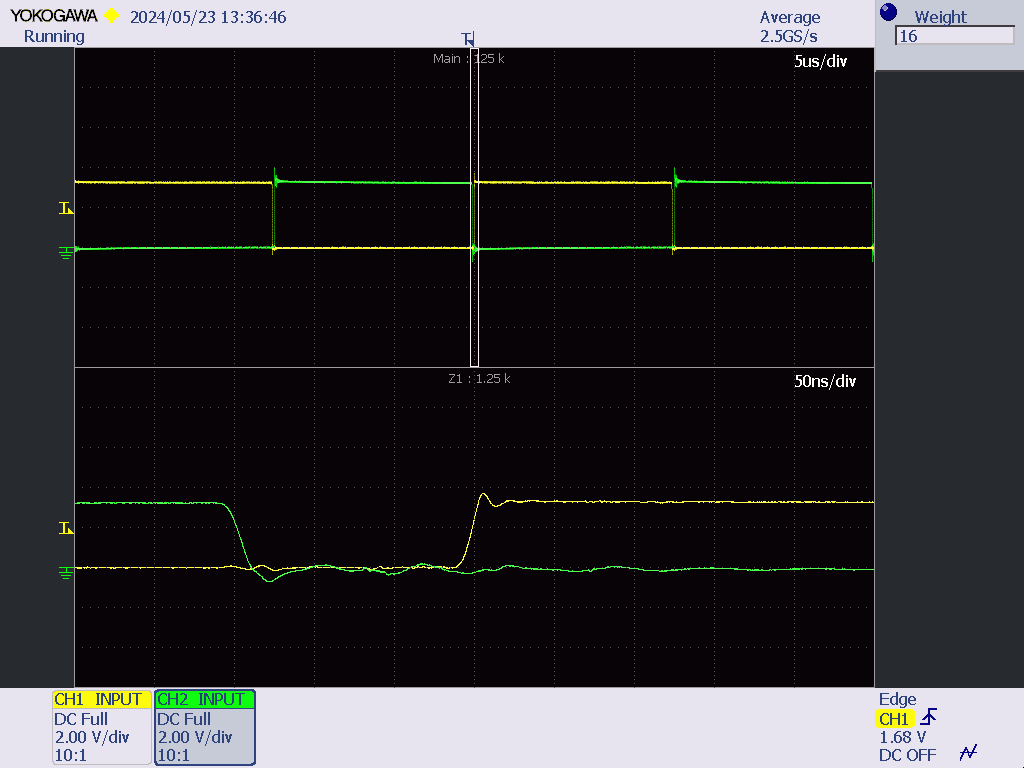
\includegraphics[width=0.7\linewidth]{fig/PWM-HSLS}
	\caption{Señales PWM a la entrada de los \textit{gate drivers}, producidas por la placa de evaluación.}
\end{figure}

\begin{figure}[H]
	\centering
	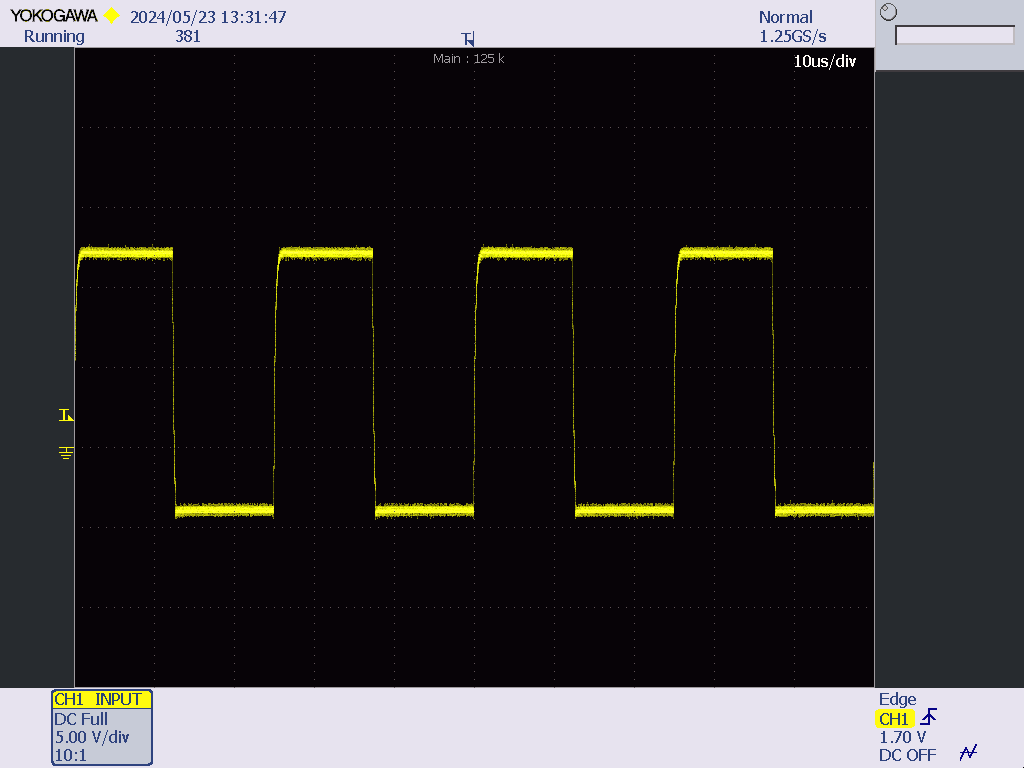
\includegraphics[width=0.7\linewidth]{fig/VGS}
	\caption{Tensión \textit{gate-source} de uno de los dos MOSFETS.}
\end{figure}


El siguiente paso fue verificar la tensión entre \textit{drain} y \textit{source}, y dado que se trata de una medida que tiene implicaciones con los parásitos del circuito, se usó una sonda con conexión \textit{pigtail} en la masa. El objetivo es minimizar el área entre la conexión a masa y la señal medida, ya que de esa forma se minimiza la inductancia equivalente total. Una medida con una inductancia alta falsearía el valor de \textit{overshoot}.


\begin{figure}[H]
	\centering
	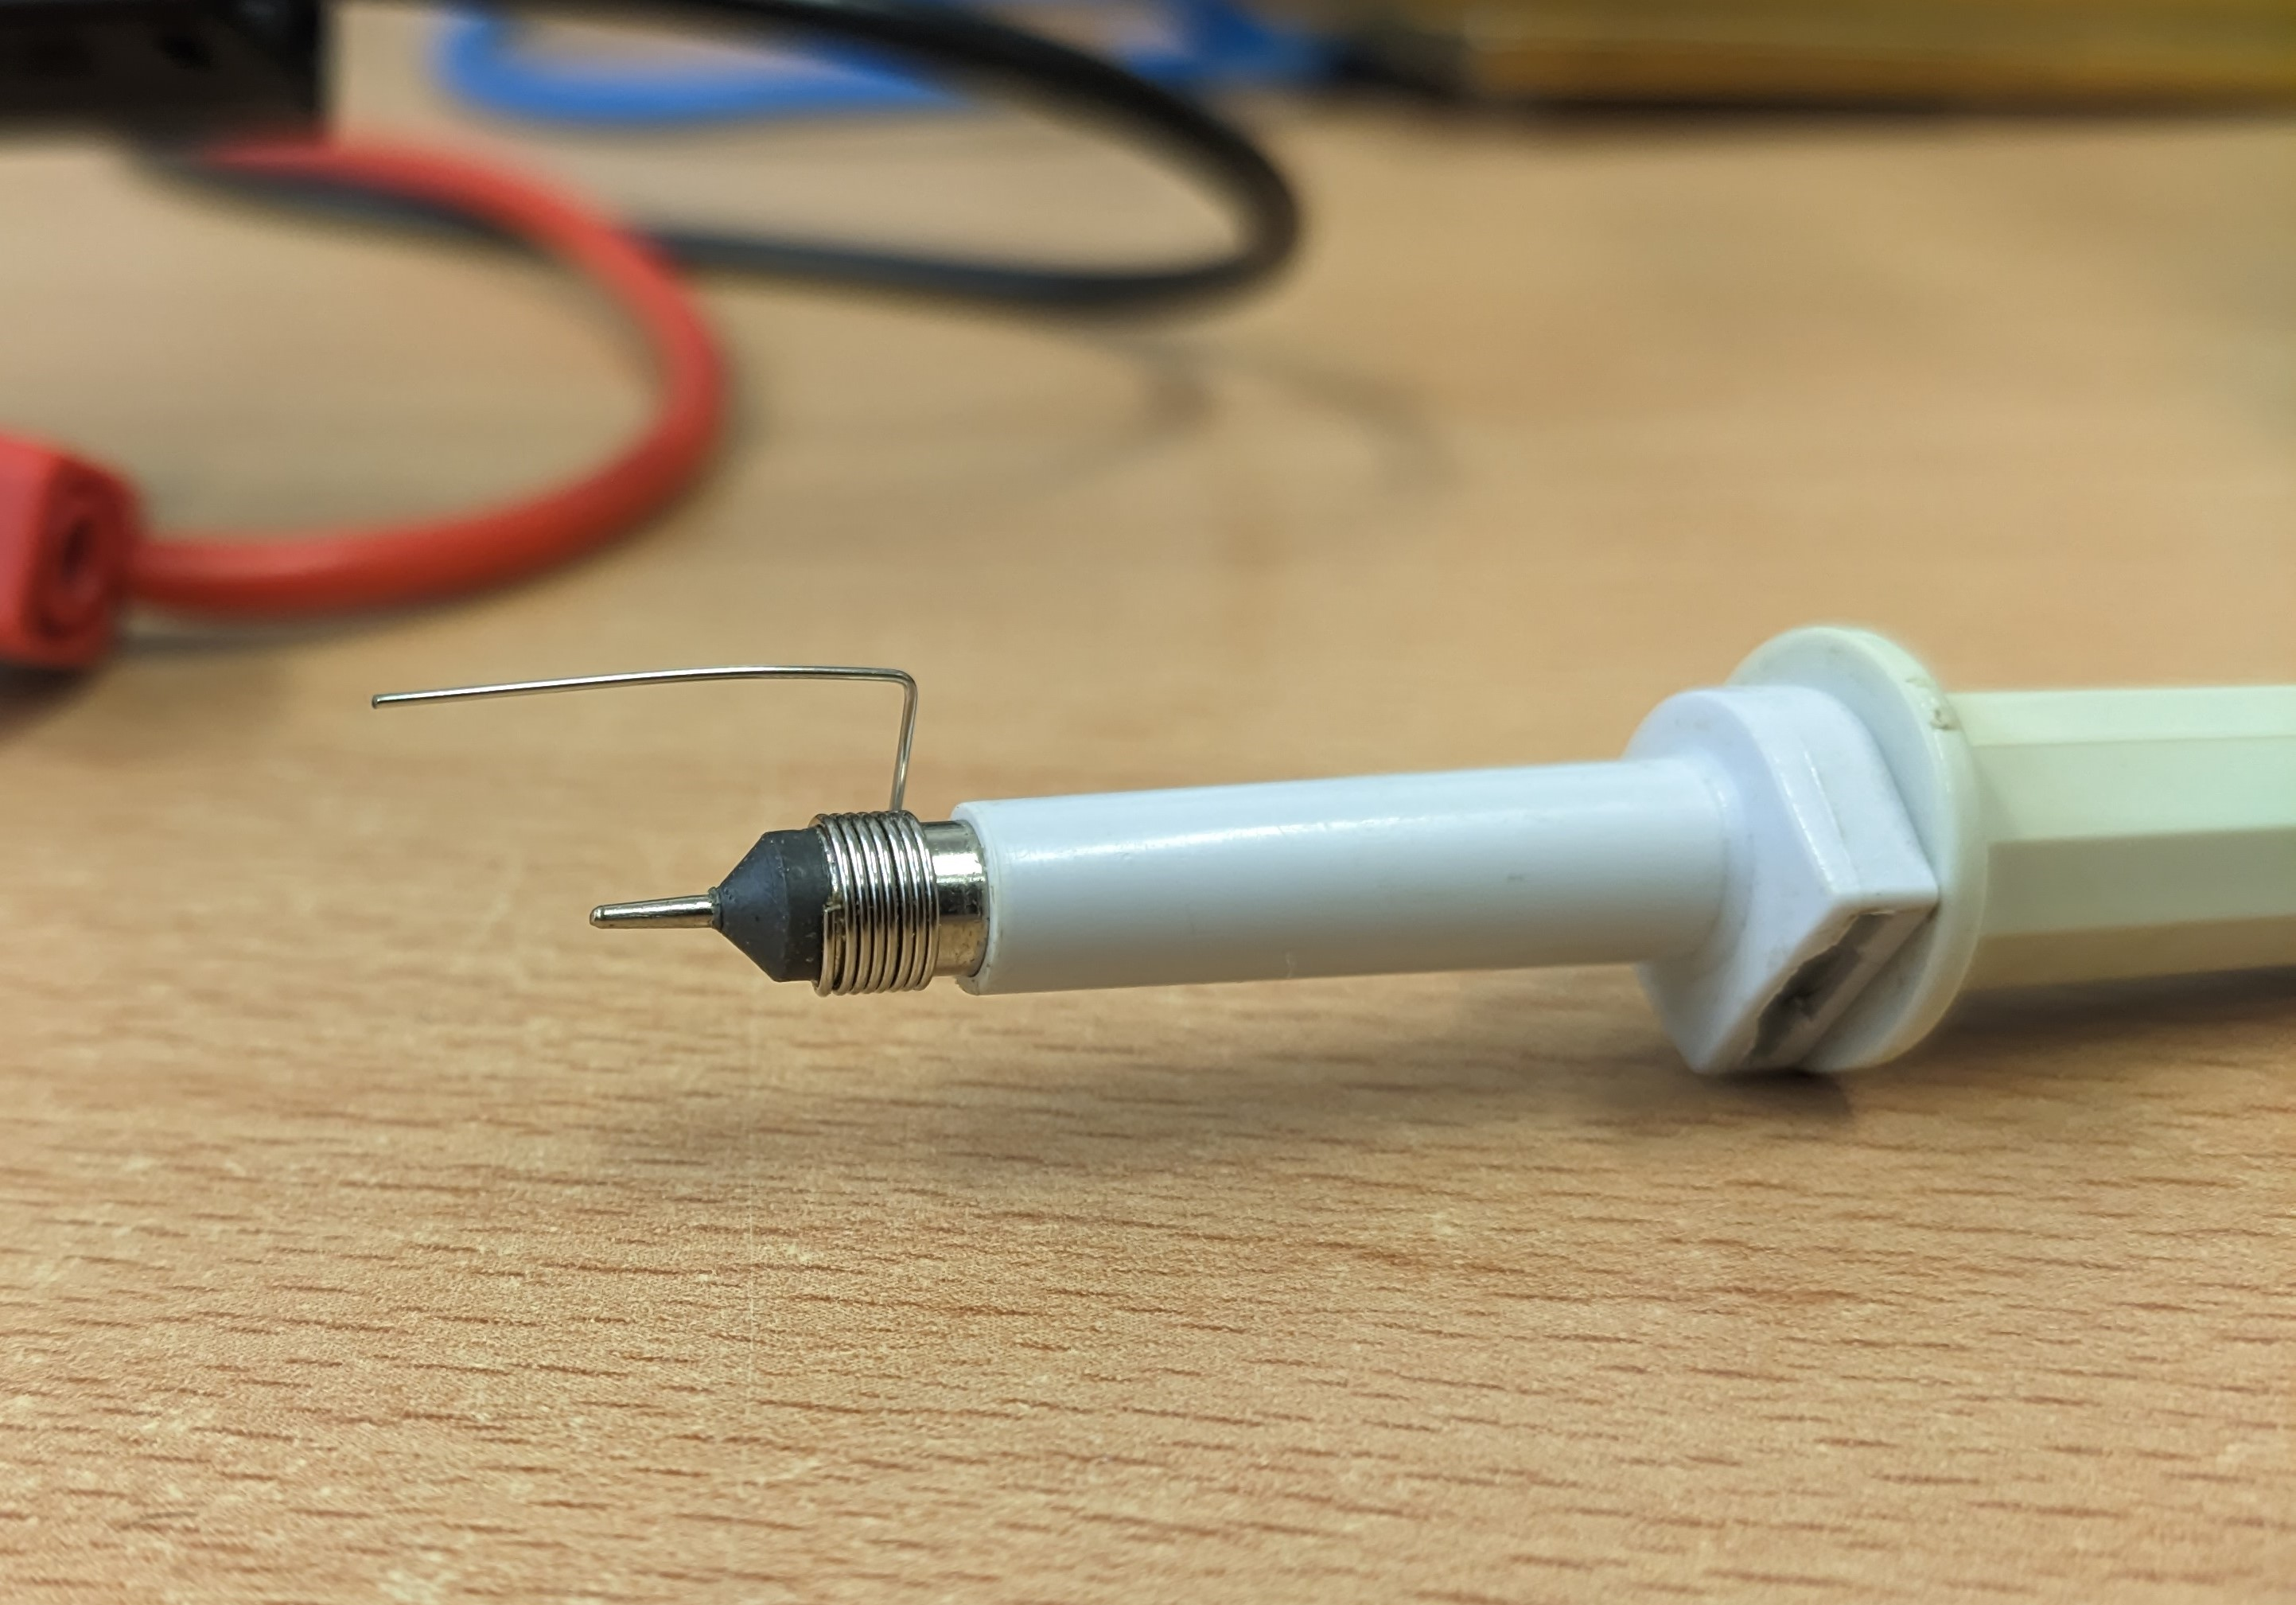
\includegraphics[width=0.7\linewidth]{fig/pigtail1}
	\caption{Sonda con \textit{pigtail}.}
\end{figure}

\begin{figure}[H]
	\centering
	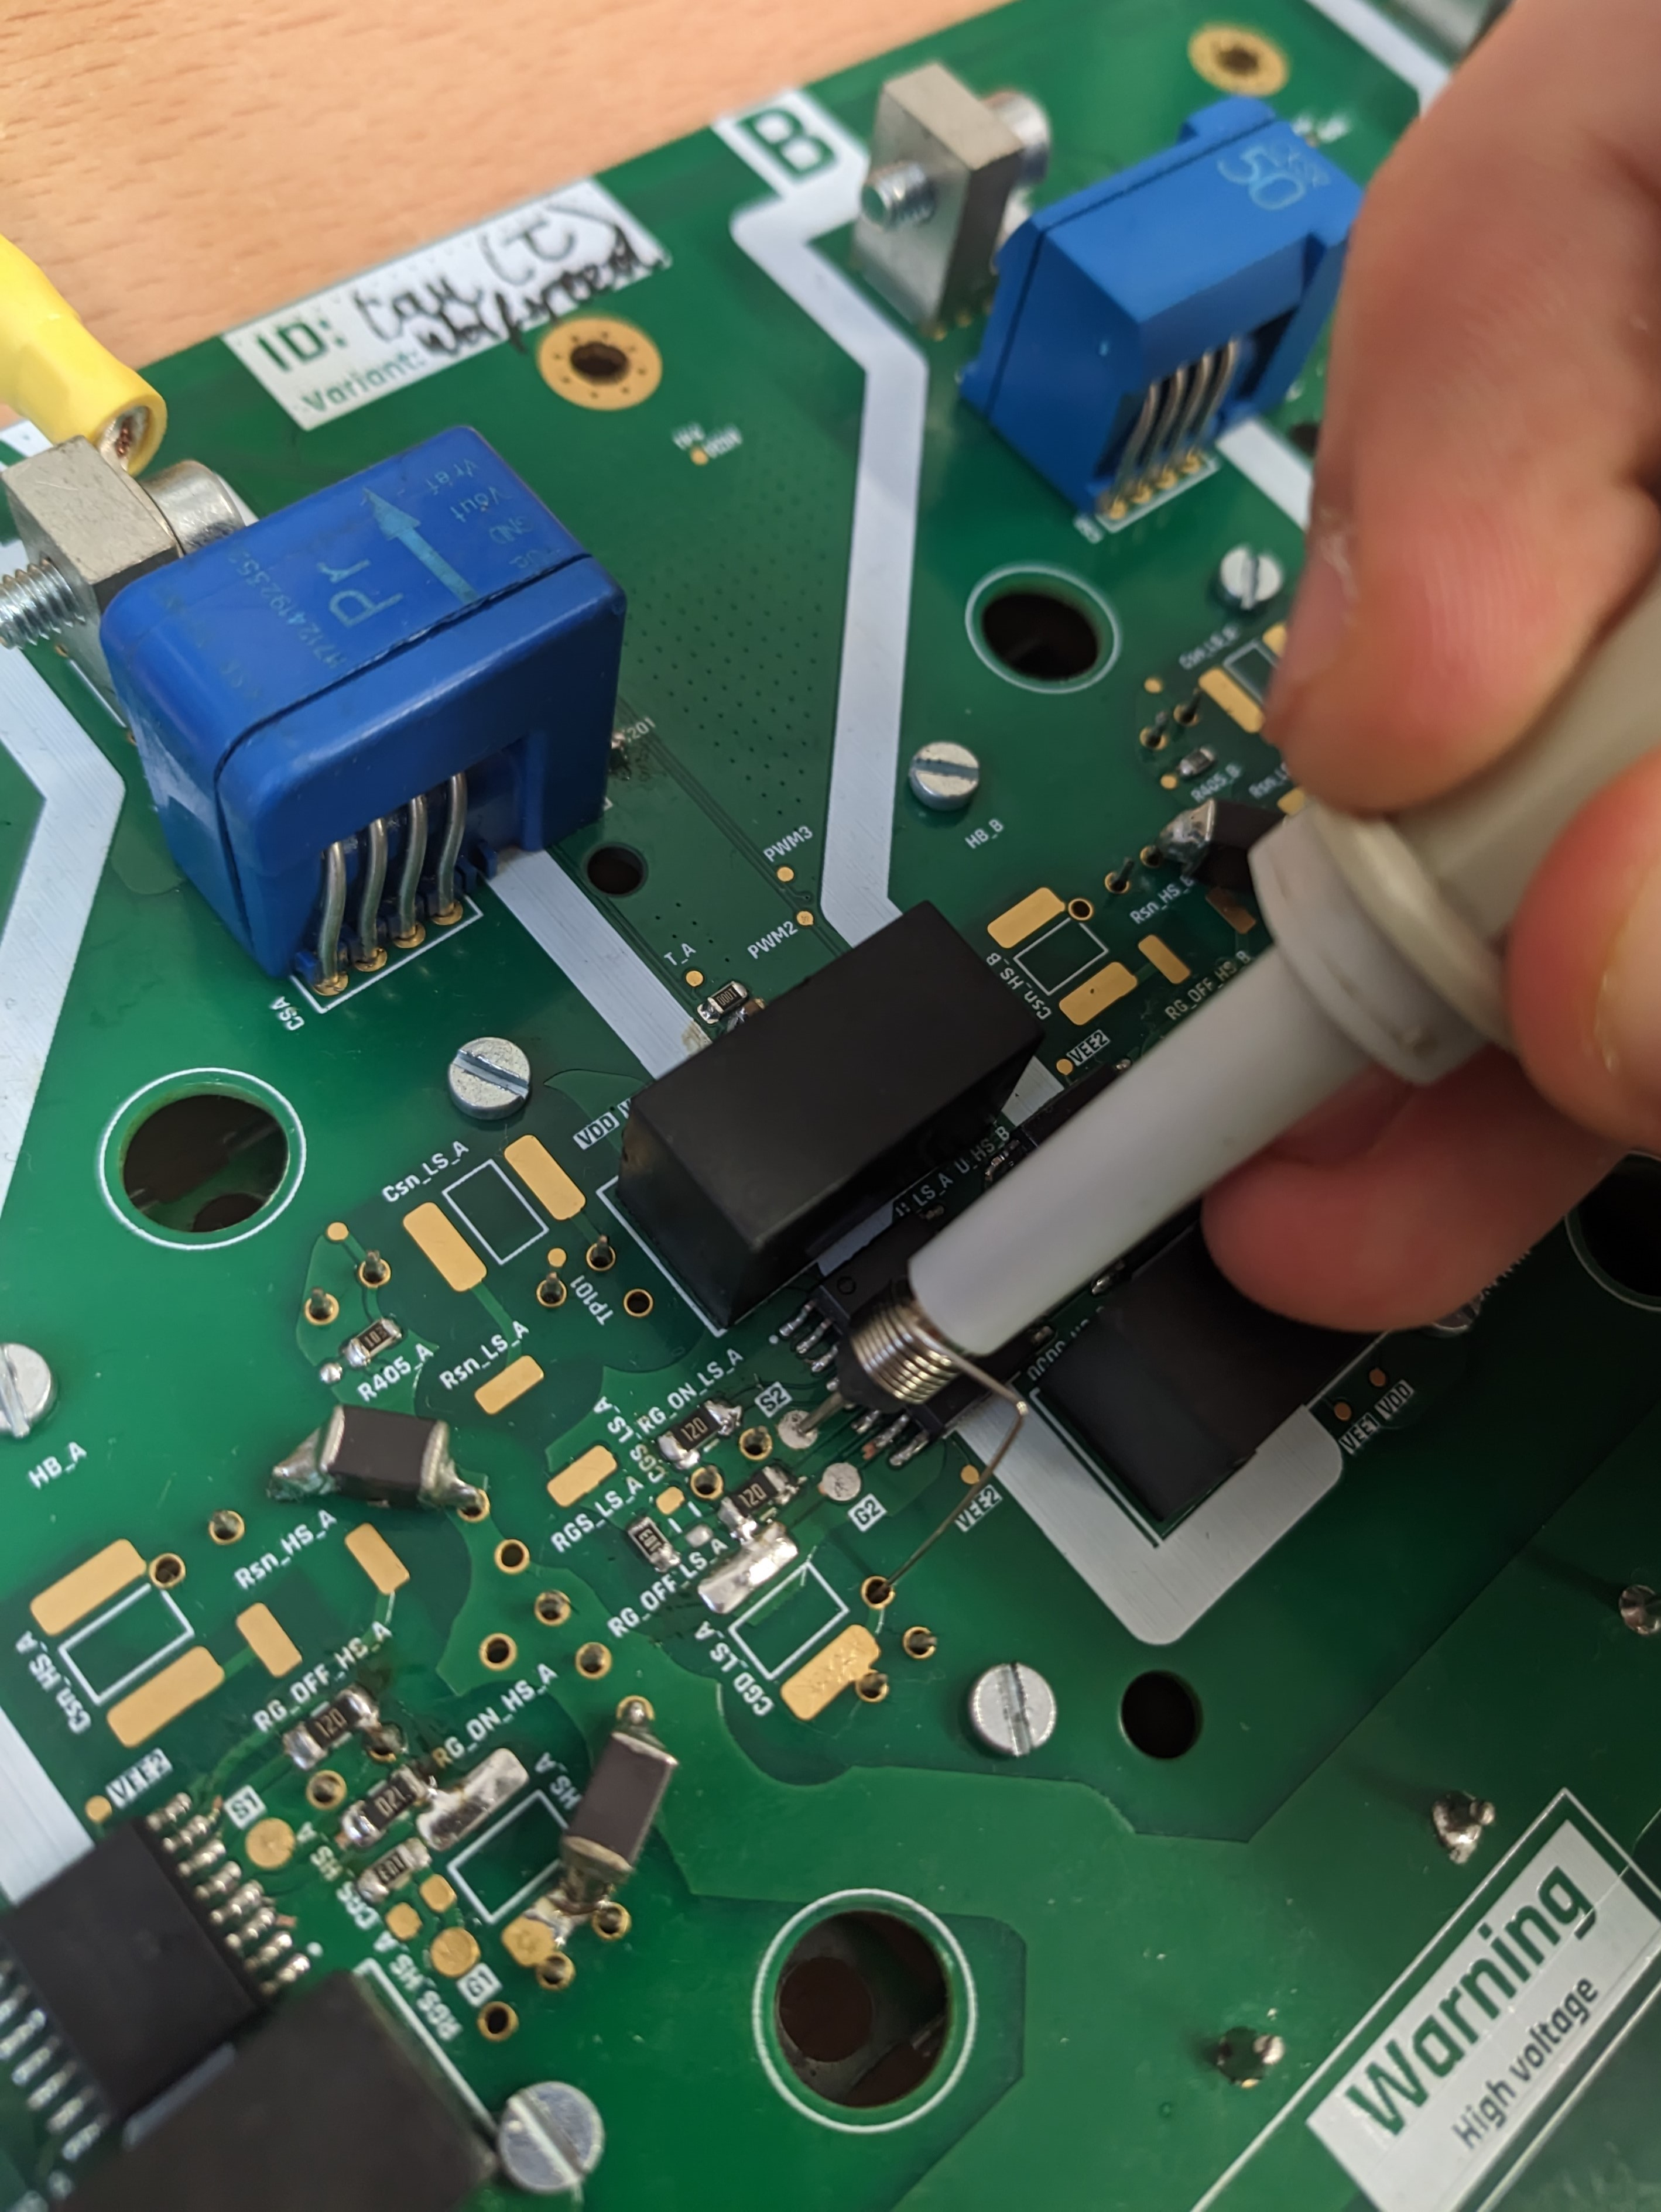
\includegraphics[width=0.45\linewidth]{fig/pigtail2}
	\caption{Medición de la tensión \textit{drain - source} (fotografía tomada posteriormente al ensayo).}
\end{figure}

Para poder observar el rizado provocado por la carga inductiva se decidió bajar la frecuencia de conmutación a 10 kHz. Posteriormente, se hizo una primera prueba con 10 V de entrada, y se observó un \textit{overshoot} muy grande.

\begin{figure}[H]
	\centering
	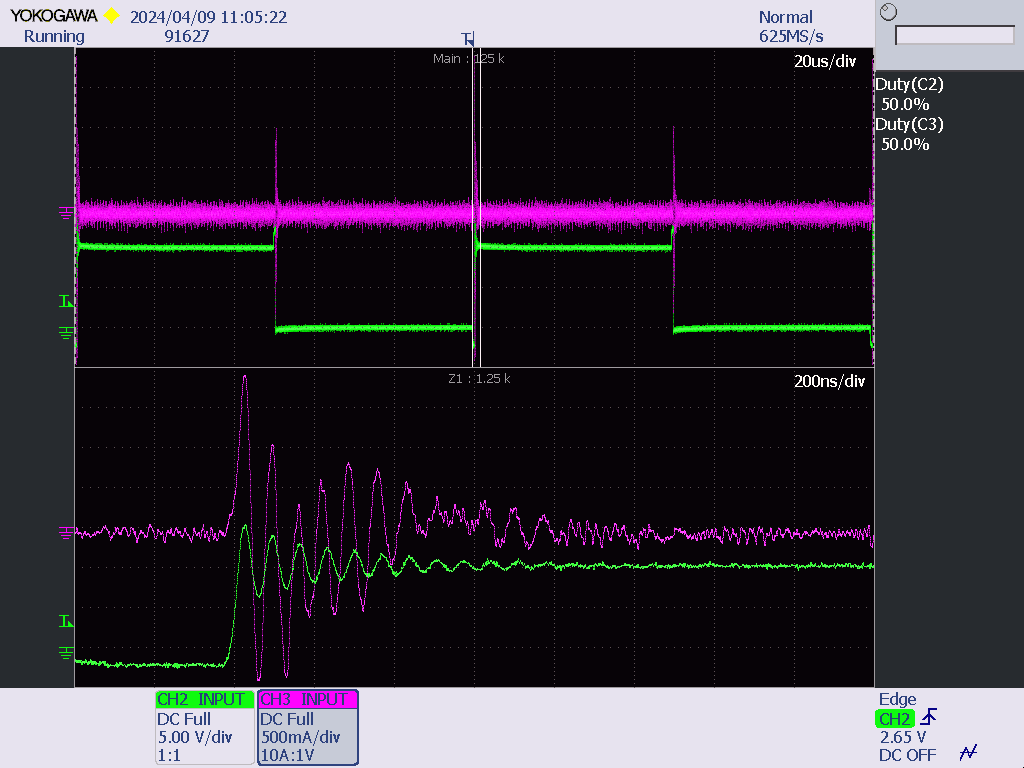
\includegraphics[width=0.7\linewidth]{fig/overshootInicial1}
	\caption{\textit{Overshoot} observado con 10 V de entrada y 0 A de salida (en vacío).}
\end{figure}

\begin{figure}[H]
	\centering
	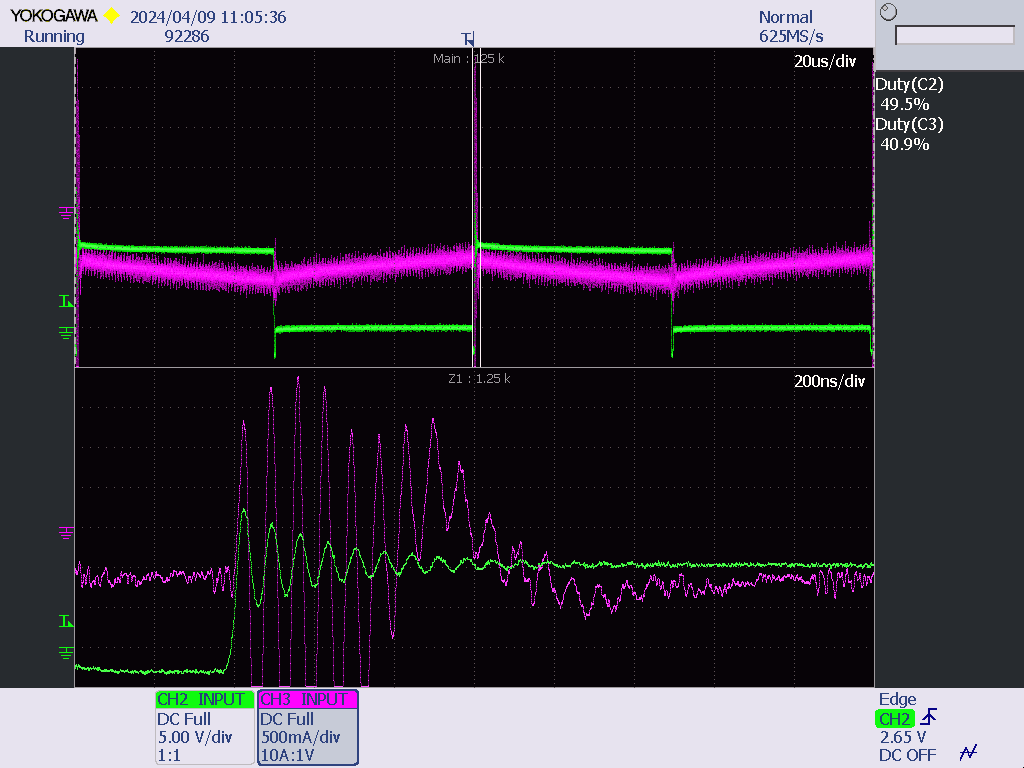
\includegraphics[width=0.7\linewidth]{fig/overshootInicial2}
	\caption{\textit{Overshoot} observado con 10 V de entrada y 0,75 A de salida (con la carga R-L).}
\end{figure}

Dado que este \textit{overshoot} es aproximadamente lineal con la corriente de salida y la tensión de entrada, se creó un modelo lineal para predecir el \textit{overshoot} a las especificaciones máximas del convertidor. Para ello se tomó un dato más a 20 V de entrada y sin carga. El resultado del modelo lineal se muestra a continuación.

\begin{table}[H]
	\centering
	\begin{tabular}{|c|c|c|c|}
		\hline
		\multicolumn{2}{|c|}{\textbf{Modelo}} & \multicolumn{2}{|c|}{$Overshoot = a \cdot V_{\text{DC,in}} + b \cdot I_{\text{out}} + c$} \\
		\hline
		\multicolumn{4}{|c|}{\textbf{Coeficientes}} \\
		\hline
		\multicolumn{2}{|c|}{$a$} & \multicolumn{2}{c|}{$1.5$} \\
		\multicolumn{2}{|c|}{$b$} & \multicolumn{2}{c|}{$6.6667$} \\
		\multicolumn{2}{|c|}{$c$} & \multicolumn{2}{c|}{$3.9721 \cdot 10^{-15}$} \\
		\hline
		\multicolumn{4}{|c|}{\textbf{Datos medidos y predicción}} \\
		\hline
		{$V_{\text{DC,in}}$} & $I_{\text{out}}$ & \textit{Overshoot} medido & Predicción de \textit{overshoot}\\
		\hline
		{$10$ V} & $0$ A & $15$ $\text{V}_p$ & $15$ $\text{V}_p$\\
		{$20$ V} & $0$ A & $30$ $\text{V}_p$ & $30$ $\text{V}_p$\\
		{$10$ V} & $0.75$ A & $20$ $\text{V}_p$ & $20$ $\text{V}_p$ \\
		\hline
		\multicolumn{4}{|c|}{Predicción de \textit{overshoot} a $600$ V y $80$ A: {\color{red}\textbf{$1433$ $\text{V}_p$}}} \\
		\hline
	\end{tabular}
	\caption{Resumen de resultados del modelo de \textit{overshoot}.}
\end{table}



\begin{figure}[H]
	\centering
	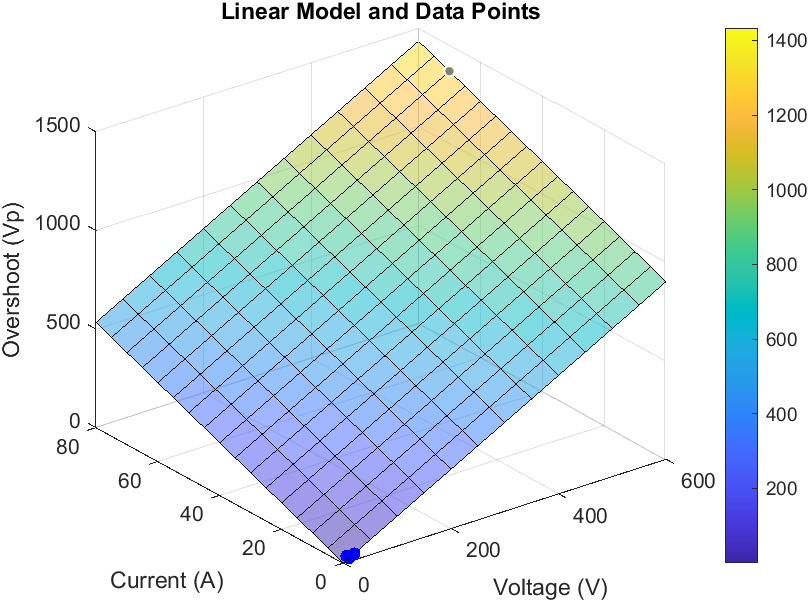
\includegraphics[width=0.7\linewidth]{fig/overshootInicial3}
	\caption{Modelo lineal (plano) junto a los datos tomados (puntos azules).}
\end{figure}

La predicción de 1433 $\text{V}_p$ es muy preocupante, ya que en primer lugar, los semiconductores serían los primeros en dañarse ya que solo aguantan 1200 V, y además, tensiones tan altas podrían provocar rupturas dieléctricas. Por tanto, es necesario reducir este \textit{overshoot}. La solución consiste en incorporar desacoplos de la conmutación entre los terminales positivo y negativo, lo más cerca posible de cada módulo \textit{half-bridge}. Interesa tener el máximo de capacidad con una resistencia serie equivalente muy baja, con lo que se descartan los condensadores electrolíticos. Se escogieron condensadores cerámicos puesto que tienen una densidad de capacidad bastante grande, mucho más alta que los condensadores de película. Sin embargo, los cerámicos tienen una pérdida de capacidad por \textit{DC bias} muy agresiva, es decir, la capacidad real es mucho baja  cuando se sube la tensión a la que se somete el condensador. Por suerte, existen gamas de condensadores pensados para estas aplicaciones que ofrecen un \textit{derating} por \textit{DC bias} bastante bajo. En este caso se escogieron los 2220Y1K00104KZT de la gama Hiteca de Knowles Syfer.

\begin{figure}[H]
	\centering
	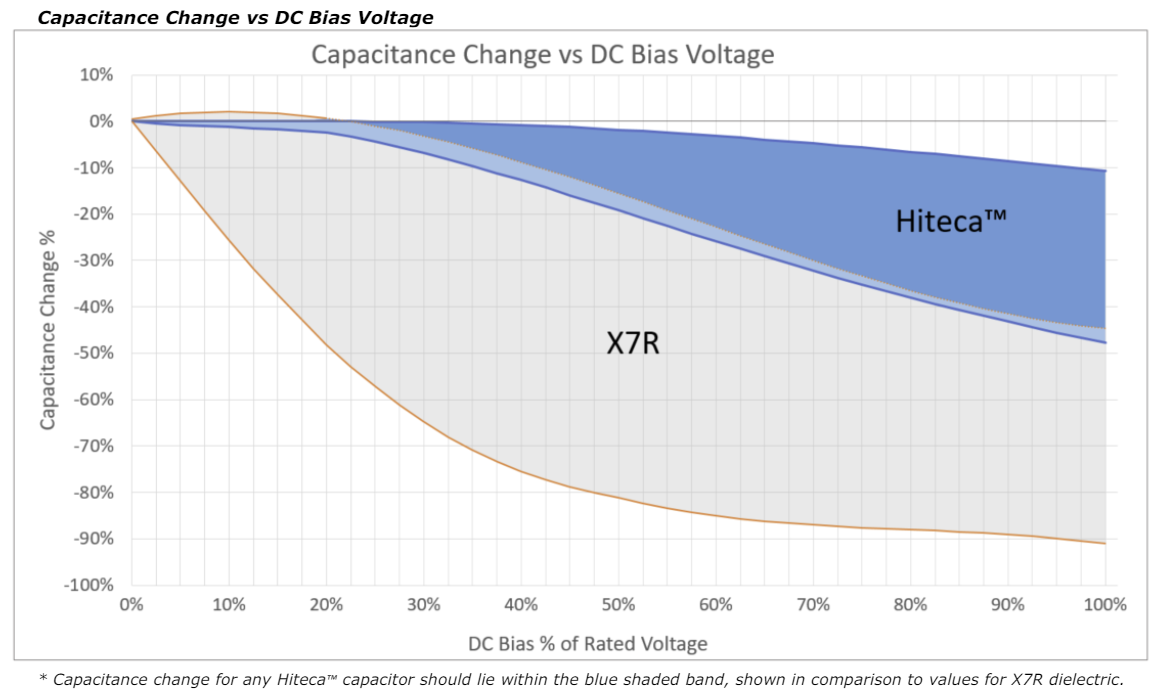
\includegraphics[width=0.7\linewidth]{fig/hiteca}
	\caption{Comparativa de la pérdida de capacidad de un condensador con aislante X7R estándar vs. el aislante usado en la gama Hiteca de Knowles Syfer \cite{KnowlesCapacitors}.}
\end{figure}

Estos condensadores son muy caros, ya que no solo el aislante es mucho mejor, sino que pueden aguantar hasta 1 kV e integran una capacidad de 100 nF en un encapsulado 2220. Se instalaron dos condensadores en cada módulo de potencia. Para esta aplicación, tan solo se perdería un 25\% de la capacidad, es decir, a 600 V no se tendrán 200 nF si no 150 nF, que ya es bastante. El \textit{rework} quedó de la siguiente manera:


\begin{figure}[H]
	\centering
	\includegraphics[width=0.7\linewidth]{fig/reworkOvershoot}
	\caption{Instalación de los condensadores de desacoplo usando los pines de los módulos de potencia.}
\end{figure}

Se volvieron a realizar las pruebas con 10 V de entrada, y se observó una reducción muy drástica del \textit{overshoot}, verificando que es una solución adecuada.

\begin{figure}[H]
	\centering
	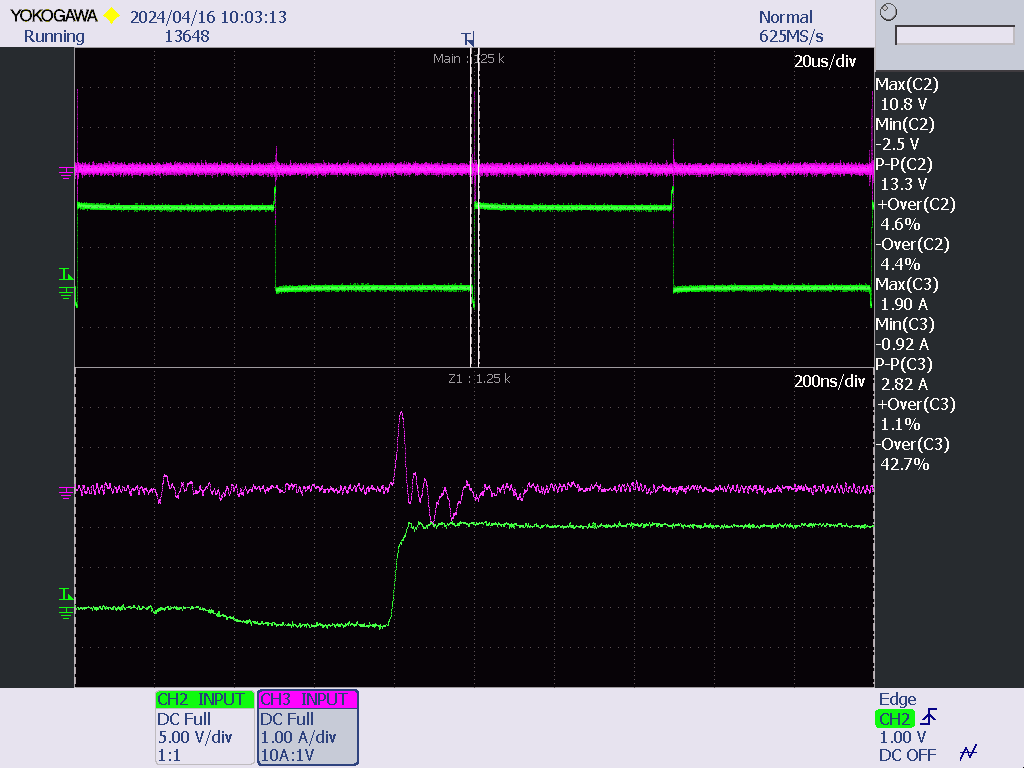
\includegraphics[width=0.7\linewidth]{fig/overshootFinal1}
	\caption{\textit{Overshoot} observado con 10 V de entrada y 0 A de salida (en vacío).}
\end{figure}

\begin{figure}[H]
	\centering
	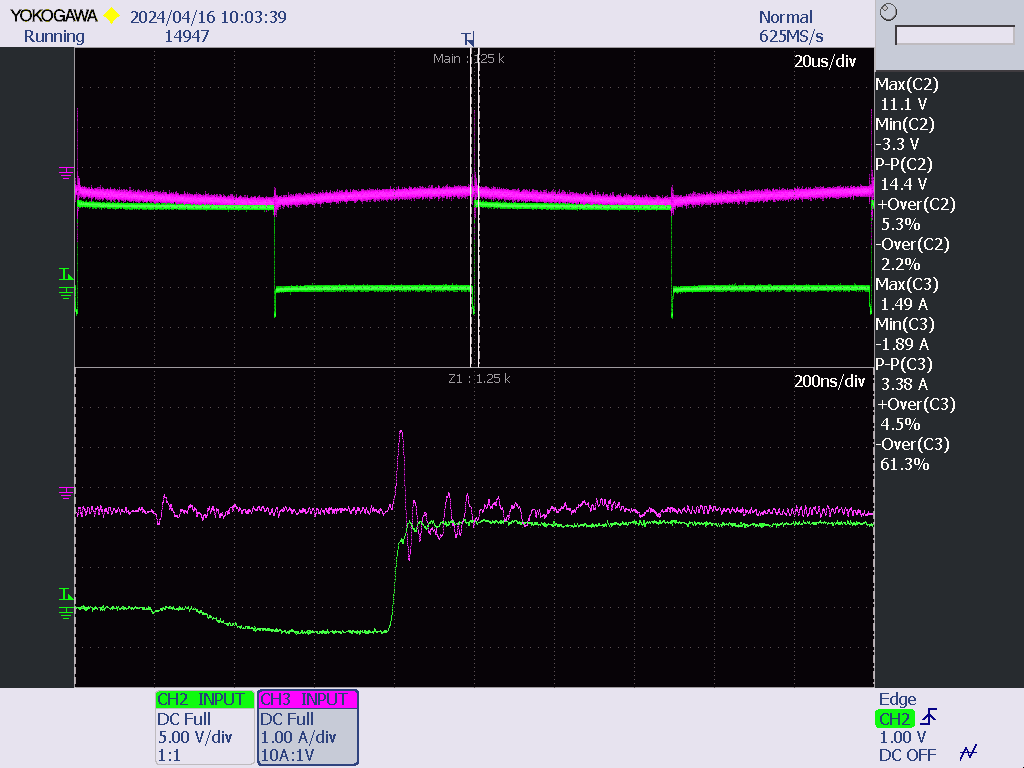
\includegraphics[width=0.7\linewidth]{fig/overshootFinal2}
	\caption{\textit{Overshoot} observado con 10 V de entrada y 0,75 A de salida (con la carga R-L).}
\end{figure}

Se creó un nuevo modelo lineal para realizar la predicción de \textit{overshoot} a las especificaciones máximas, y en este caso, se tomaron muchos más puntos, siendo la fuente de alimentación con la que se ensayó el factor limitante para no poder tomar más.

\begin{figure}[H]
	\centering
	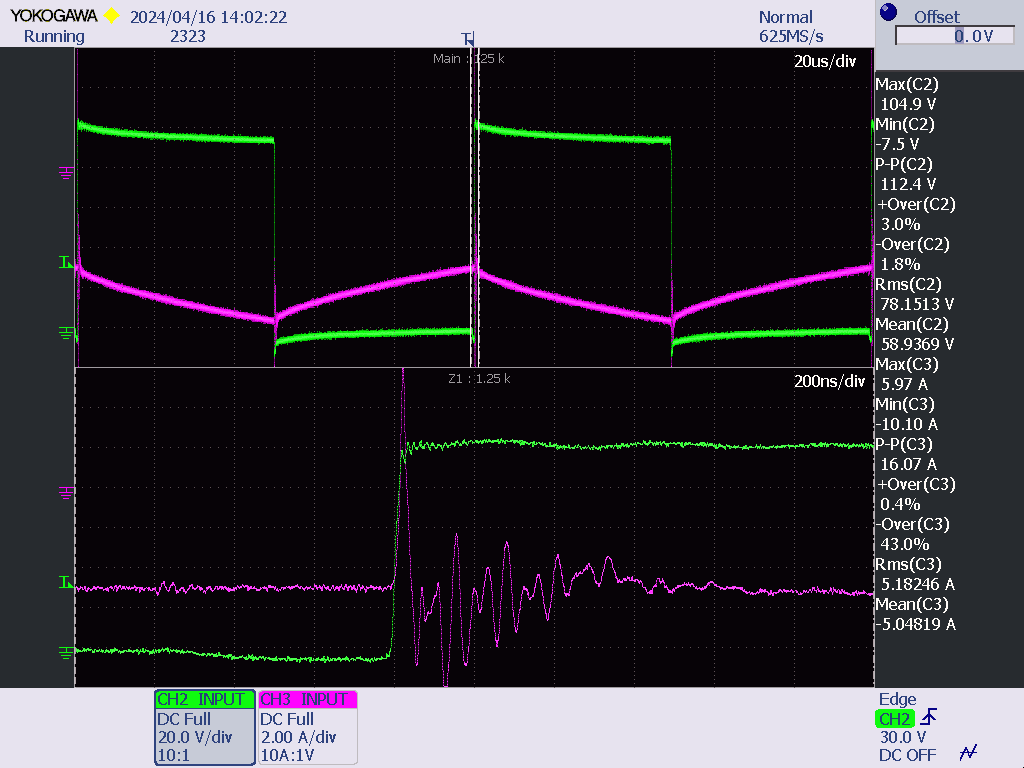
\includegraphics[width=0.7\linewidth]{fig/overshootFinal4}
	\caption{\textit{Overshoot} observado con 90 V de entrada y 6,2 A de salida (con la carga R-L).}
\end{figure}

\begin{table}[H]
	\centering
	\begin{tabular}{|c|c|c|c|}
		\hline
		\multicolumn{2}{|c|}{\textbf{Modelo}} & \multicolumn{2}{|c|}{$Overshoot = a \cdot V_{\text{DC,in}} + b \cdot I_{\text{out}} + c$} \\
		\hline
		\multicolumn{4}{|c|}{\textbf{Coeficientes}} \\
		\hline
		\multicolumn{2}{|c|}{$a$} & \multicolumn{2}{c|}{$1.1463$} \\
		\multicolumn{2}{|c|}{$b$} & \multicolumn{2}{c|}{$0.42886$} \\
		\multicolumn{2}{|c|}{$c$} & \multicolumn{2}{c|}{$-1.3001$} \\
		\hline
		\multicolumn{4}{|c|}{\textbf{Datos medidos y predicción}} \\
		\hline
		$V_{\text{DC,in}}$ & $I_{\text{out}}$ & \textit{Overshoot} medido & Predicción de \textit{overshoot} \\
		\hline
		$10$ V & $0$ A & $10.8$ $\text{V}_p$ & $10.1626$ $\text{V}_p$ \\
		$10$ V & $0.75$ A & $11.1$ $\text{V}_p$ & $10.4843$ $\text{V}_p$ \\
		$20$ V & $0$ A & $21.3$ $\text{V}_p$ & $21.6254$ $\text{V}_p$ \\
		$20$ V & $1.5$ A & $21.5$ $\text{V}_p$ & $22.2687$ $\text{V}_p$ \\
		$30$ V & $0$ A & $31.7$ $\text{V}_p$ & $33.0882$ $\text{V}_p$ \\
		$30$ V & $2.25$ A & $32.3$ $\text{V}_p$ & $34.0531$ $\text{V}_p$ \\
		$40$ V & $0$ A & $45.9$ $\text{V}_p$ & $44.551$ $\text{V}_p$ \\
		$40$ V & $3$ A & $46.9$ $\text{V}_p$ & $45.8375$ $\text{V}_p$ \\
		$80$ V & $5.5$ A & $92.6$ $\text{V}_p$ & $92.7608$ $\text{V}_p$ \\
		$90$ V & $0$ A & $102.5$ $\text{V}_p$ & $101.8648$ $\text{V}_p$ \\
		$90$ V & $6.2$ A & $104.9$ $\text{V}_p$ & $104.5238$ $\text{V}_p$ \\
		$120$ V & $0$ A & $135.6$ $\text{V}_p$ & $136.2532$ $\text{V}_p$ \\
		$150$ V & $0$ A & $172$ $\text{V}_p$ & $170.6415$ $\text{V}_p$ \\
		$180$ V & $0$ A & $205$ $\text{V}_p$ & $205.0298$ $\text{V}_p$ \\
		$200$ V & $0$ A & $227$ $\text{V}_p$ & $227.9553$ $\text{V}_p$ \\
		\hline
		\multicolumn{4}{|c|}{Predicción de \textit{overshoot} a $600$ V y $80$ A: {\color{red}\textbf{$720.775$ $\text{V}_p$}}} \\
		\hline
	\end{tabular}
	\caption{Resumen de resultados del modelo de \textit{overshoot}.}
\end{table}



\begin{figure}[H]
	\centering
	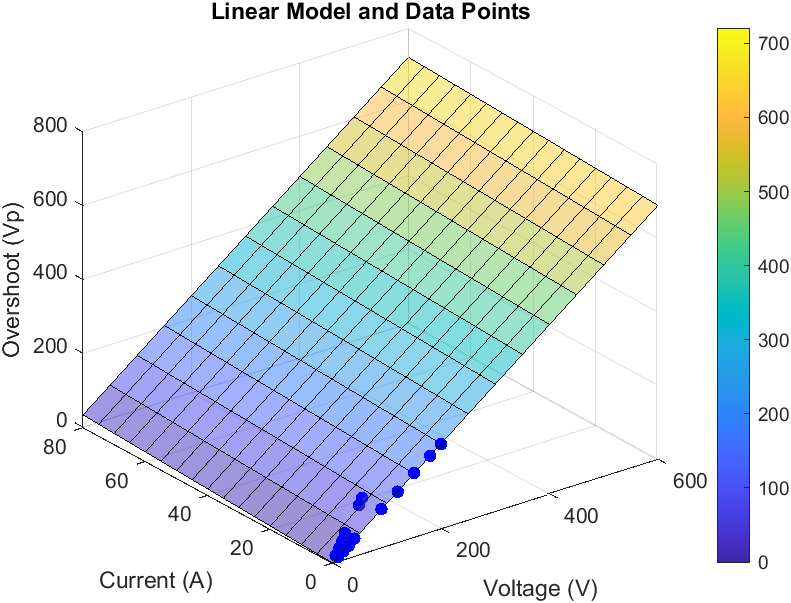
\includegraphics[width=0.7\linewidth]{fig/overshootFinal3}
	\caption{Modelo lineal (plano) junto a los datos tomados (puntos azules).}
\end{figure}

Los resultados fueron muy positivos porque el \textit{overshoot} de $720.775 \text{ V}_p$ es totalmente asumible. A estas alturas no se pudo pedir otra iteración de la PCB puesto que hubiese sido muy costoso, pero igualmente se actualizaron los esquemáticos con los desacoplos en los terminales de los semiconductores.

\begin{figure}[H]
	\centering
	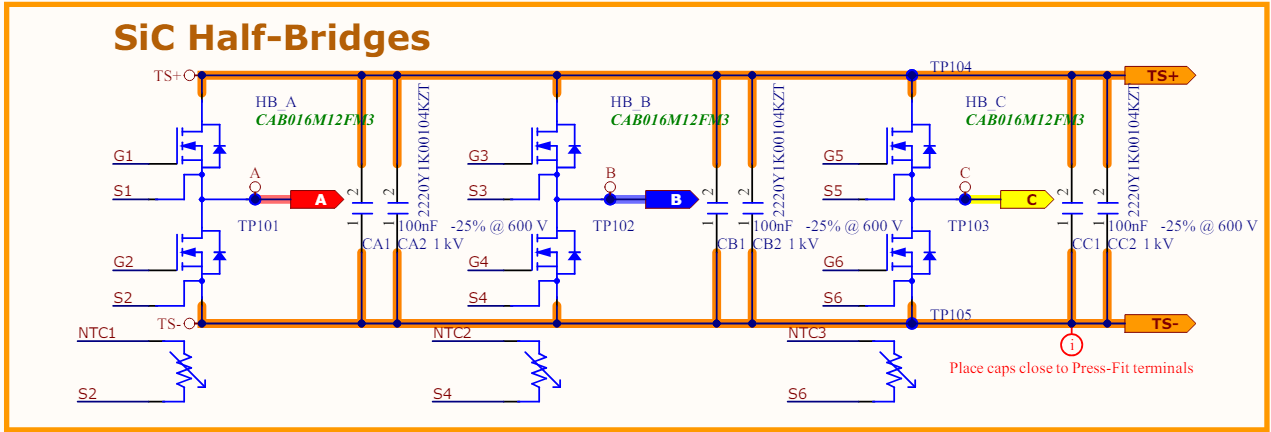
\includegraphics[width=0.7\linewidth]{fig/schPowerDecoupling}
	\caption{Esquemático de la etapa de potencia actualizado.}
\end{figure}


\subsection{Pruebas térmicas y de alta tensión}

La última prueba que se hizo a la placa de potencia fue una serie de ensayos de descarga, a cada vez más tensión. El objetivo de este test es asegurar que no se produce ninguna ruptura dieléctrica y que las resistencias de descarga son capaces de aguantar la tensión máxima permanentemente.

Para realizar estos ensayos fue necesario usar dos autotransformadores, uno de ellos aislado. El primero, monofásico, se conecta a la red normal, y el otro, a la red trifásica. Se rectificó la salida de cada uno con un puente de diodos (uno monofásico y uno trifásico), y se conectaron los dos rectificadores en serie para obtener una tensión continua de hasta 800 V. Se usaron un par de contactores, uno para realizar la precarga del bus de continua y otro para conectarlo directamente al rectificador.

Para evaluar las temperaturas se dispuso de una cámara térmica, que permitió distinguir con claridad qué partes de la PCB se calentaban más. Para capturar la tensión se usó una sonda diferencial de 1400 V.

\begin{figure}[H]
	\centering
	\begin{subfigure}[b]{0.45\textwidth}
		\centering
		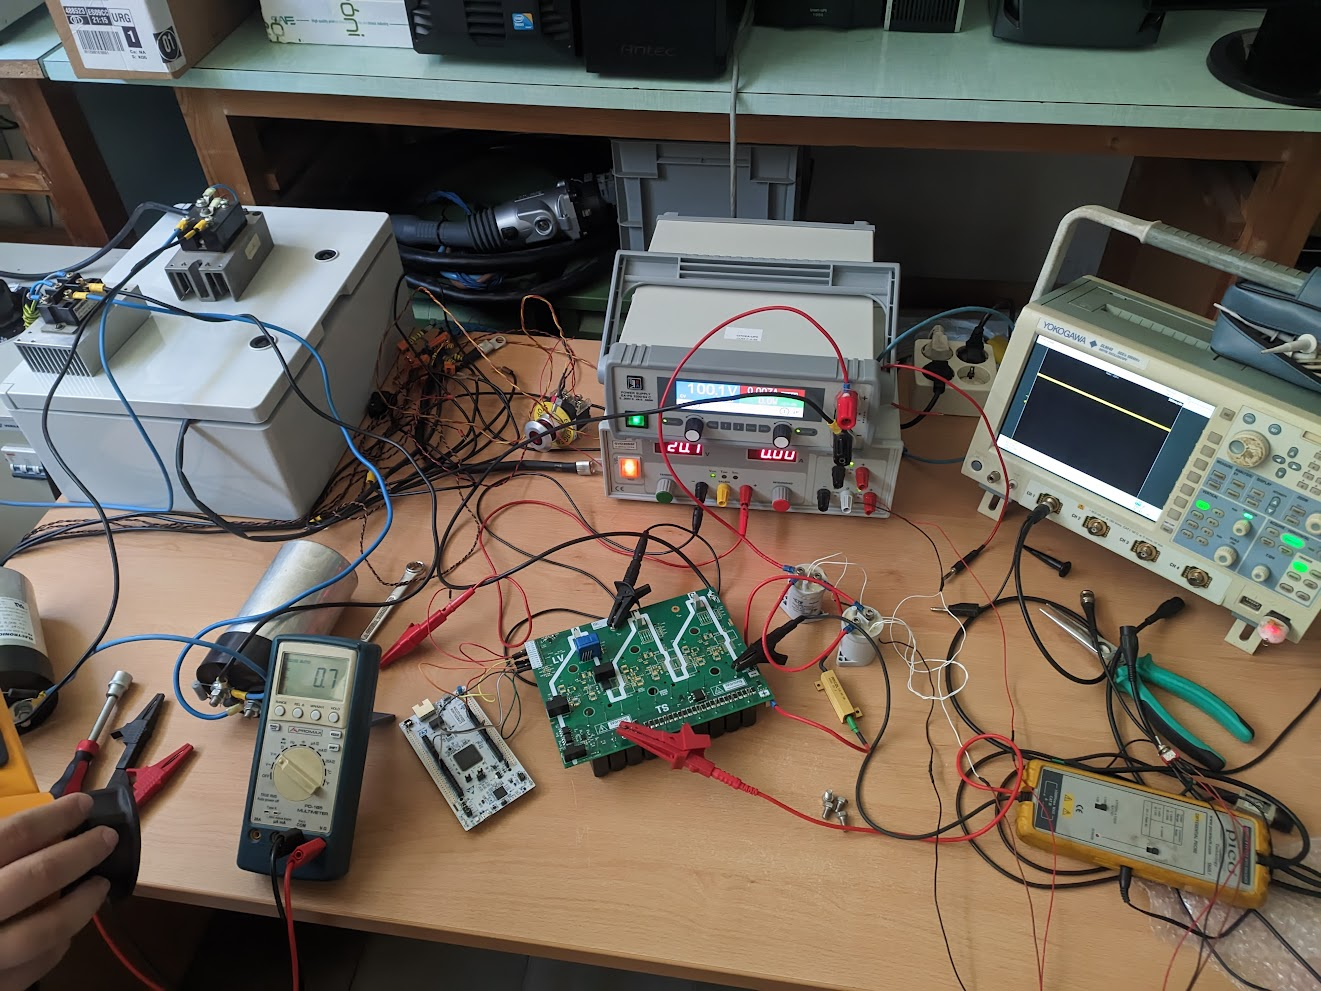
\includegraphics[width=\textwidth]{fig/setupDischarge1}
	\end{subfigure}
	\hfill
	\begin{subfigure}[b]{0.45\textwidth}
		\centering
		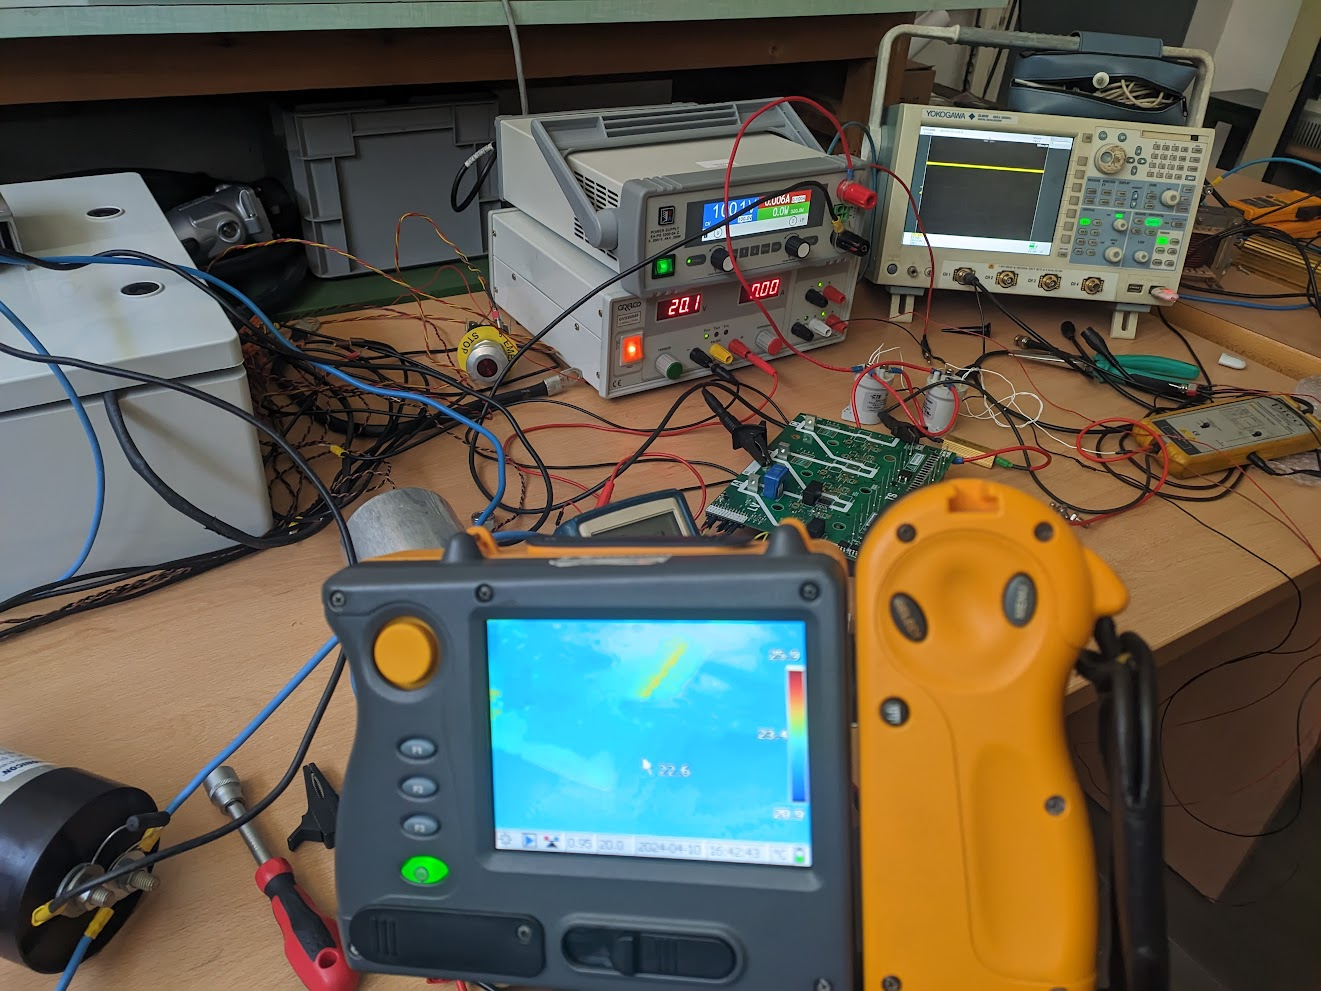
\includegraphics[width=\textwidth]{fig/setupDischarge2}
	\end{subfigure}
	\caption{Vistas del \textit{setup} para las pruebas de descarga.}

\end{figure}


Los ensayos se realizaron de la siguiente forma: 

\begin{enumerate}
	\item Se precarga el bus de continua con una resistencia de externa.
	\item Se mantiene hasta lograr el estado estacionario térmico, evaluado con una cámara térmica. En este punto, la descarga activa está desactivada y se evalúa la descarga pasiva.
	\item Se conecta la descarga activa pero se deja el contactor conectado de manera que el bus no se descarga. Se espera hasta alcanzar el estado estacionario térmico.
	\item Se abren los contactores y se descarga el bus.
\end{enumerate}

A continuación se muestra el ensayo más exigente, una descarga a 600 V.

\begin{figure}[H]
	\centering
	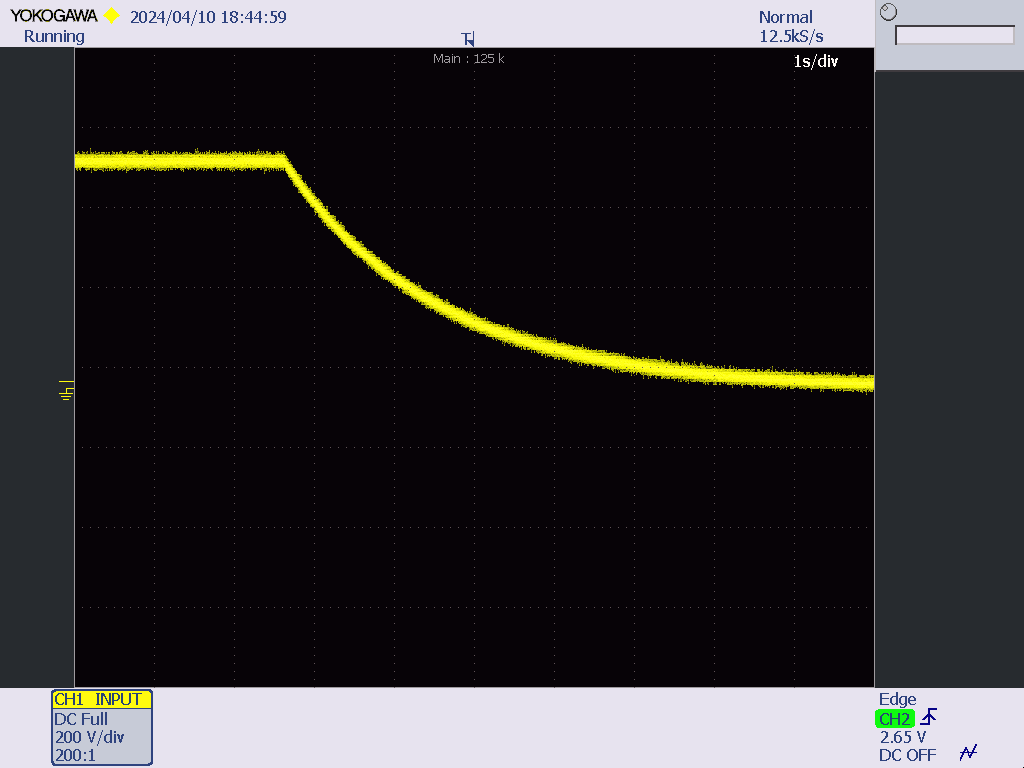
\includegraphics[width=0.7\linewidth]{fig/dischargeGuapo}
	\caption{Descarga de 600 V a 60 V con 100 \unit{\micro\farad} de capacidad en el bus de continua, en un tiempo de 4,5 segundos.}
\end{figure}

\begin{figure}[H]
	\centering
	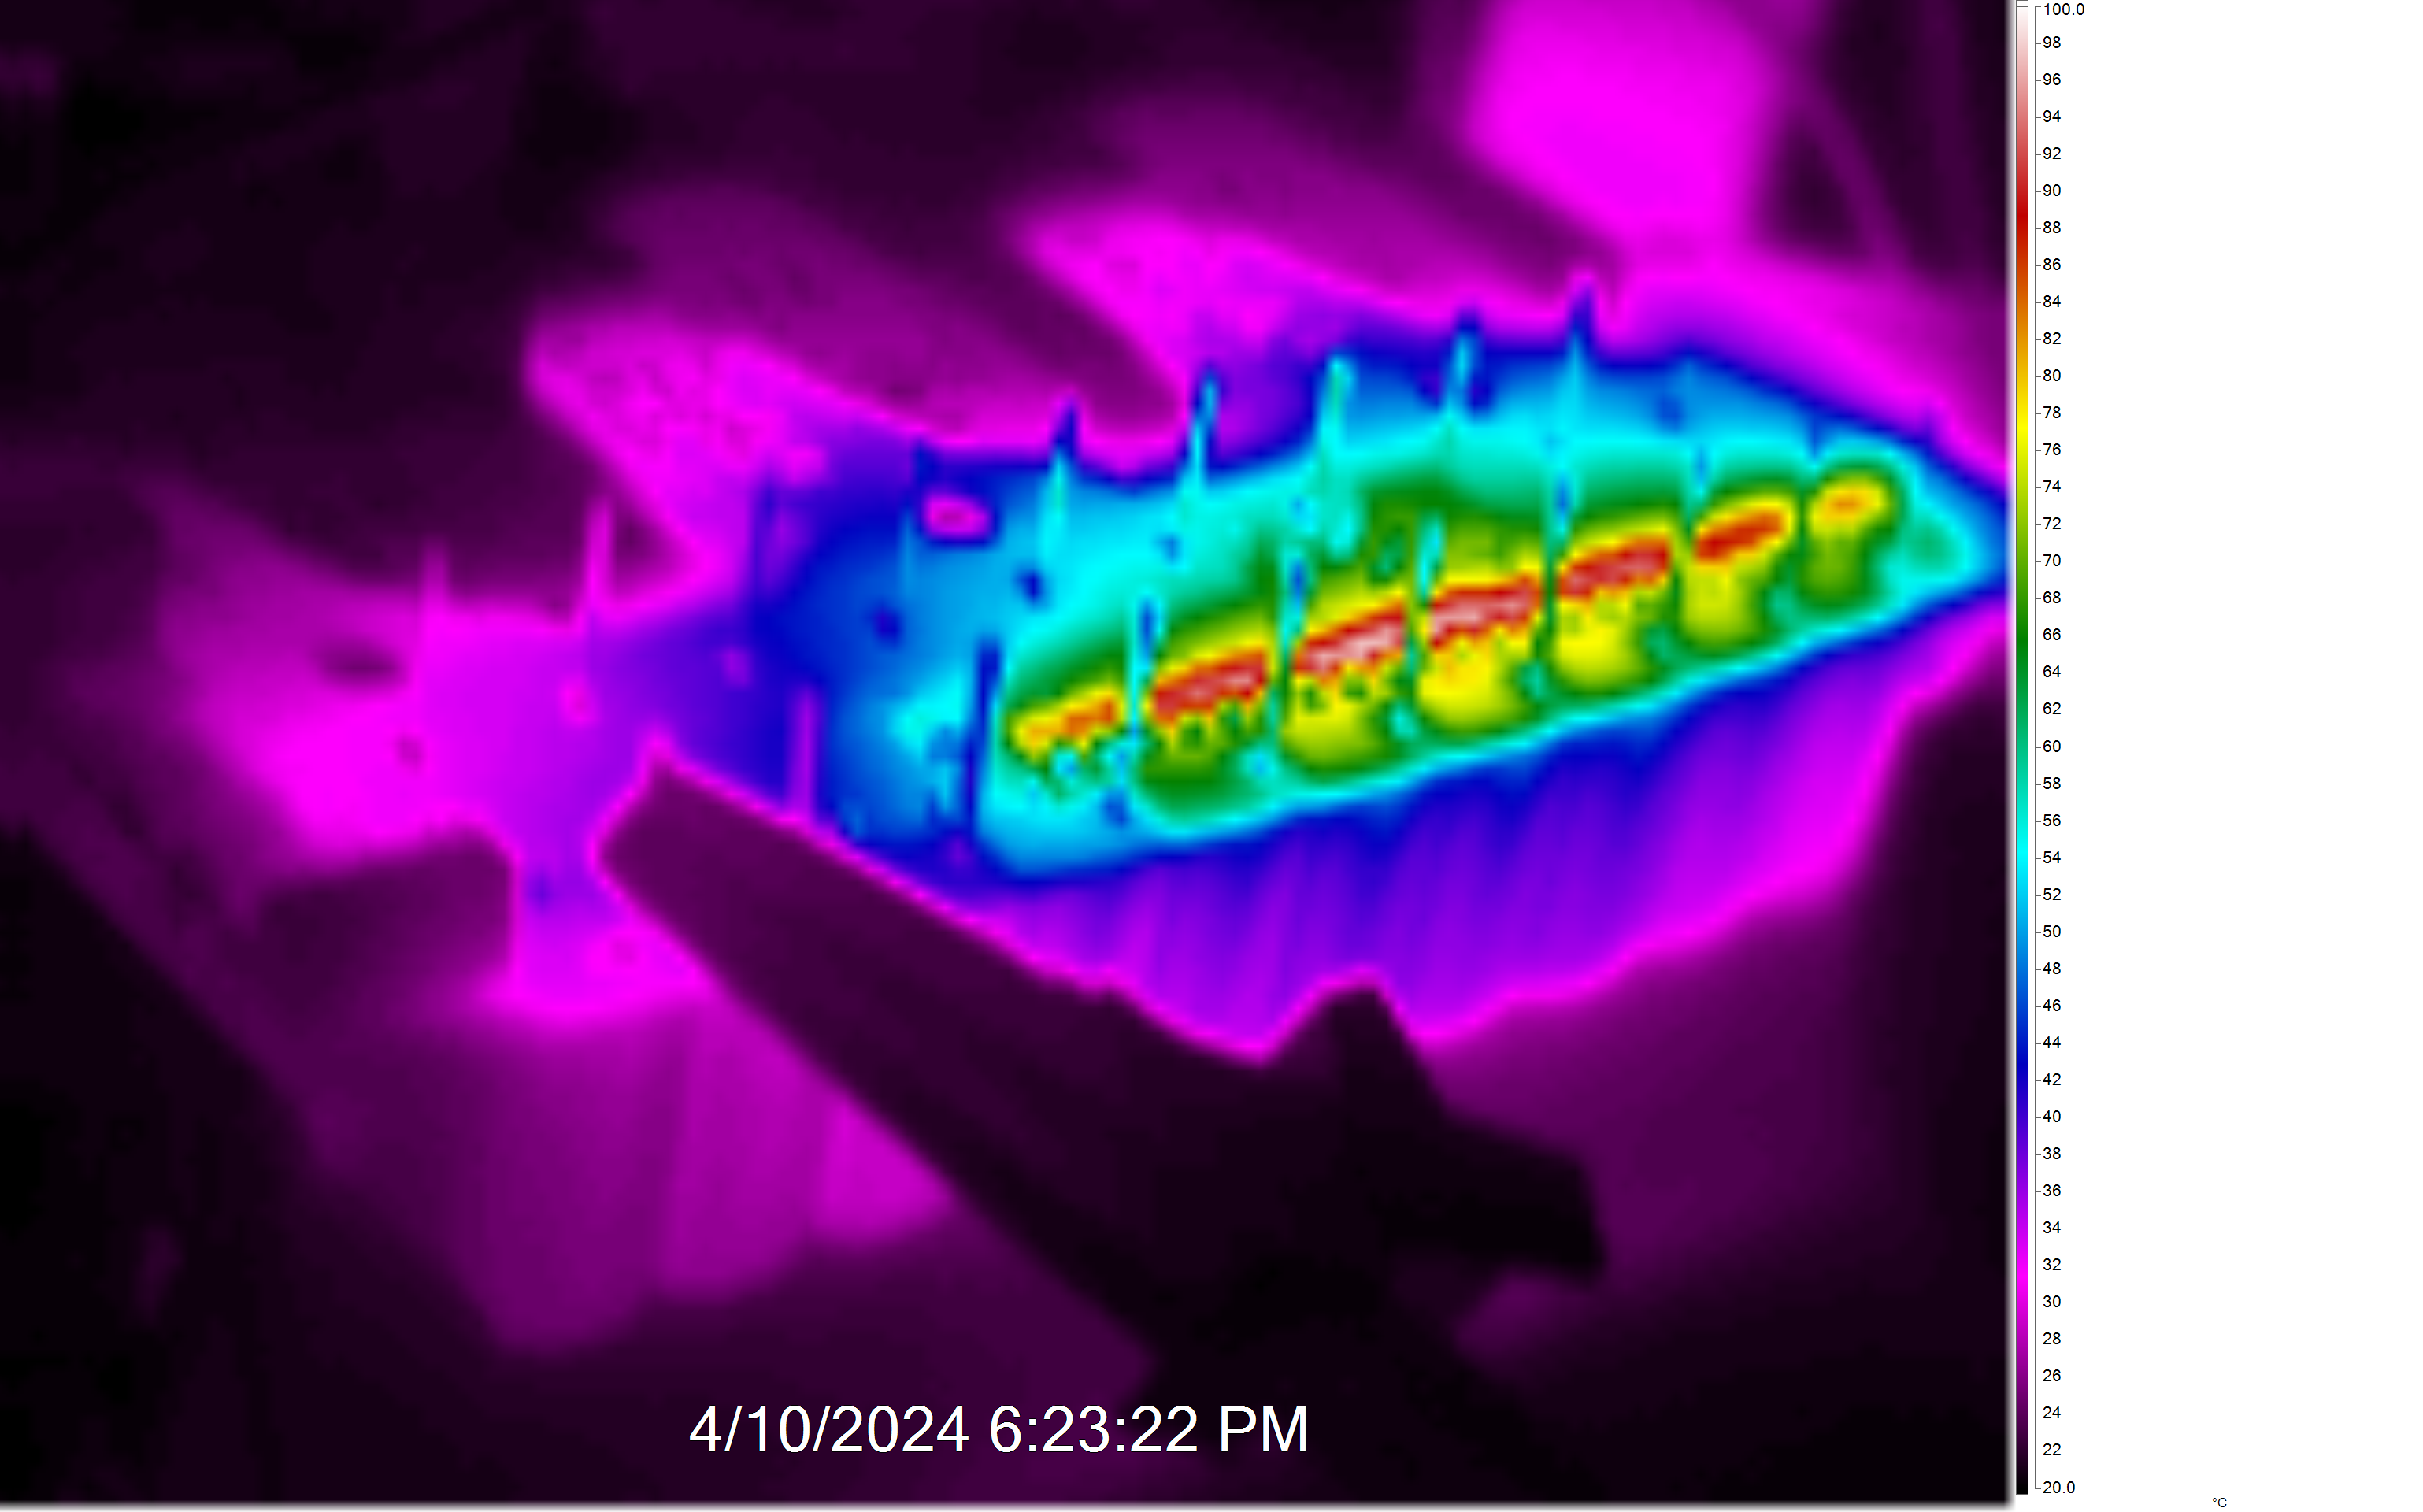
\includegraphics[width=0.7\linewidth]{fig/dischargeGuapisimo}
	\caption{Captura de la cámara térmica tras alcanzar el estado estacionario térmico a 600 V.}
\end{figure}



Se puede observar un pico de temperatura de 100 $^{\circ}$C, y la temperatura ambiente era de 25 $^{\circ}$C aproximadamente. Cada resistencia disipa $\frac{(600 \text{ V})^2}{470 \text{ k}\Omega} = 0.766 \text{ W}$, lo cual se correspondería con una resistencia térmica de aproximadamente $ \frac{100 \text{ }^{\circ}\text{C} - 25 \text{ }^{\circ}\text{C}}{0.766 \text{ W}} \approx 100 \text{ K/W}$. Este valor es muy razonable para una resistencia SMD sin \textit{pad} térmico ni mucha consideración en el \textit{layout}, de acuerdo con \cite{vishay_application_note}.

\subsection{Validación de la placa de control}

La validación de la placa de control se llevó a cabo tras la instalación inicial del \textit{hardware}, que incluyó el microcontrolador y los componentes esenciales para su funcionamiento básico. El \textit{hardware} de esta placa es relativamente sencillo en comparación con la placa de potencia, así que se destinó más tiempo a programar que a mirar detenidamente los subcircuitos de esta placa. Aunque el proceso de validación se realizó de manera preliminar y parcial, se abordaron varias áreas clave:

\subsubsection{Alimentación}

La placa se alimenta exclusivamente del sistema de baja tensión del monoplaza, con una tensión nominal entre 20 V y 30 V. Inicialmente, se tenía previsto implementar un convertidor para obtener un bus de 5 V, sin embargo, debido a la complejidad y dificultades de soldadura del convertidor, se optó por utilizar una fuente de alimentación externa de 5 V para realizar las pruebas iniciales. De todas maneras, el convertidor es de Recom, una marca con la que el equipo ha trabajado varios años y se confía en la calidad de sus convertidores. Sin embargo, se vio que la bobina del filtro Pi (L101) no tiene el \textit{rating} de corriente suficiente. Se deberá escoger una bobina que pueda soportar más corriente en una siguiente versión de la placa.

\subsubsection{MCU}

El MCU seleccionado fue el STM32F777VI, que se integra como el bloque central de la placa. La prioridad fue lograr programarlo por primera vez, que se logró con éxito no mucho después de montarlo. Por suerte, antes de montarlo por primera vez, se detectaron algunos errores en el diseño inicial de la PCB, con lo que se evitó soldarlo en esta primera versión. Estos errores son:
\begin{itemize}
	\item El pin \textit{BOOT0} (pin 94 del MCU) debe estar conectado a GND utilizando una resistencia de 10 k$\Omega$ o un valor similar.
	\item Las pistas del bus I$^2$C de la EEPROM deben tener resistencias de \textit{pull-up} cuyo valor debe determinarse según la velocidad del bus.
	\item El filtro de alimentación debería estar en el bus de 5 V en vez de en el de 20-30 V.
	\item El pin \textit{Vbat} debe estar conectado a 3.3 V.
\end{itemize}

Para abordar estos errores, se realizaron las siguientes modificaciones en \textit{Inverter\_Control}:

\begin{itemize}
	\item Se agregaron resistencias de \textit{pull-up} y \textit{pull-down} para controlar \textit{BOOT0}.
	\item Se añadieron resistencias de \textit{pull-up} para las líneas I$^2$C.
	\item Se eliminó la conexión \textit{LV+\_sns} y se conectó \textit{Vbat} a 3.3 V.
	\item Se realizaron cambios en el color y nombres de los LEDs para mayor claridad.
	\item Se trasladó el filtro de alimentación al bus de 5 V.
	\item Se realizaron ajustes en el serigrafiado.
\end{itemize}

Estas modificaciones corrigieron los errores detectados en \textit{Inverter\_Control} y permitieron un desarrollo adecuado.

\subsubsection{CAN}

El bloque CAN, que incluye un transceptor para la comunicación con el vehículo, ha sido probado con éxito. Tras configurar con éxito el periférico, se importó la base de datos de mensajes y señales y se programó la información a enviar y recibir.

\subsubsection{Retroalimentación}

Aunque se han integrado conexiones para el \textit{encoder} incremental y el \textit{front-end} analógico de la lectura de temperatura del motor, las pruebas se han limitado principalmente a las lecturas en el MCU. Esto se debe a que no se ha dispuesto del motor con el que se usará este inversor, pero por suerte los subcircuitos son muy simples y se ha podido verificar la lectura desde el MCU con señales externas.

\subsubsection{\textit{Front-end} analógico de la placa de potencia}

El \textit{front-end} analógico, que trata las señales de las placas de potencia para adaptarlas a los rangos de tensión admitidos por los ADCs del MCU, presenta algunos desafíos. Mientras que las lecturas de corriente y temperatura se han validado con éxito, la lectura de tensión mediante un amplificador diferencial no funcionó como se esperaba. La integración del circuito integrado no fue buena, y, aunque fue simulado mediante SPICE adecuadamente, los resultados no coincidieron con lo esperado. La solución implementada consistió en conectar directamente el negativo de la señal diferencial a GND y el positivo a la entrada del ADC. De todas formas, se insta a buscar una alternativa más elegante. Se están considerando otras posibilidades, como obtener la lectura de tensión a través del bus CAN, que podría ser proporcionada directamente por la batería del vehículo. Esto sería viable ya que realmente esta medida sirve como límite para evitar sobremodular, y la dinámica eléctrica de una batería es muy lenta.
.

\section{Validación de \textit{firmware}}

\subsection{Conmutación de las tres ramas}

Tras configurar correctamente los periféricos necesarios, el siguiente paso es la conmutación de las tres ramas simultáneamente, siendo el siguiente paso desde los ensayos como \textit{buck} síncrono con una sola rama. Realmente lo único necesario fue portar el \textit{firmware} de la placa de evaluación a la placa de control y activar la salida de los otros dos canales (y sus respectivos negados).

% foto PWM 3 fases

\subsection{Lazo abierto de tensión con carga R-L}

Posteriormente se implementó la modulación SVPWM y las transformadas inversas para poder consignar una tensión alterna. Usando una fuente de tensión limitada por corriente como bus de continua, se conectó una carga R-L trifásica estática a los terminales de las fases del convertidor. El valor de las inductancias utilizadas es de unos 500 \unit{\micro\henry}, y el de las resistencias de 0,5 $\Omega$. El valor real de la carga resistiva, sin embargo, se sitúa entorno a los 0,8 $\Omega$ si se tienen en cuenta las resistencias de los cables y conexiones.

\begin{figure}[H]
	\centering
	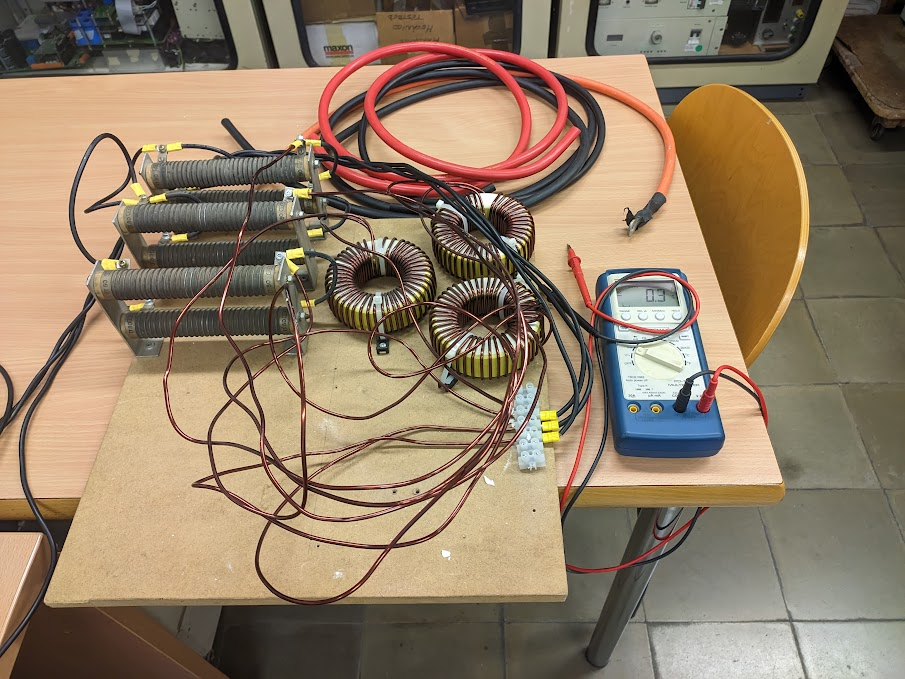
\includegraphics[width=0.7\linewidth]{fig/3RL-load}
	\caption{Carga R-L trifásica utilizada.}
\end{figure}

\begin{figure}[H]
	\centering
	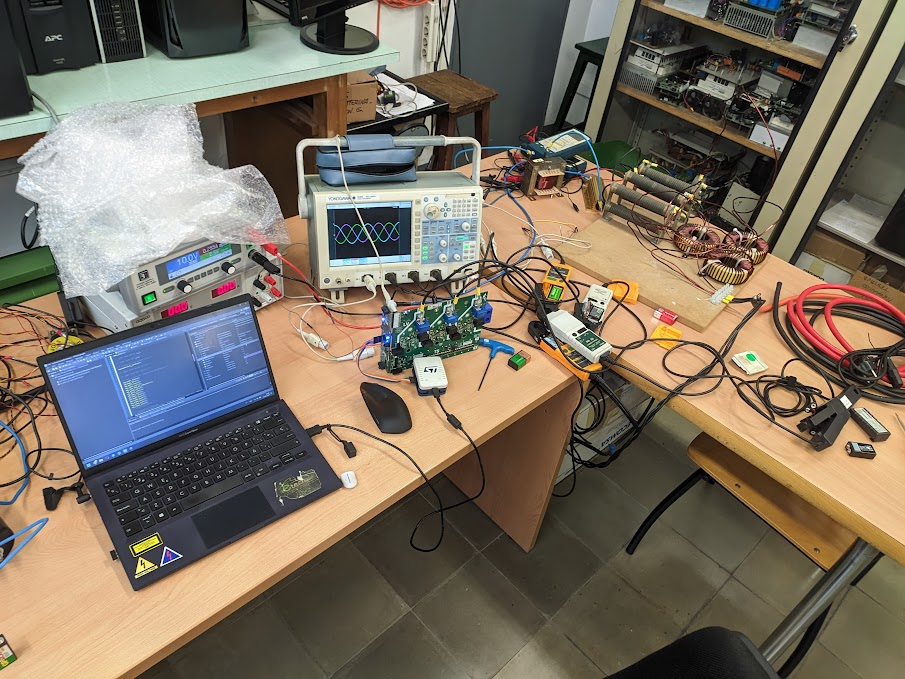
\includegraphics[width=0.7\linewidth]{fig/3RL-setup}
	\caption{\textit{Setup} del ensayo con carga R-L.}
\end{figure}

En primer lugar, y con una frecuencia de conmutación muy baja (5 kHz), se sintetizó una frecuencia de 500 Hz (relación de portadora a modulada de 10). Con esto se puede verificar el ensanchamiento y estrechamiento de los tres canales PWM reflejando las tres señales senoidales desfasadas 120 grados, generadas por la modulación SVPWM. Además, al ser una frecuencia de conmutación tan baja, se puede apreciar el rizado en la corriente de salida.

\begin{figure}[H]
	\centering
	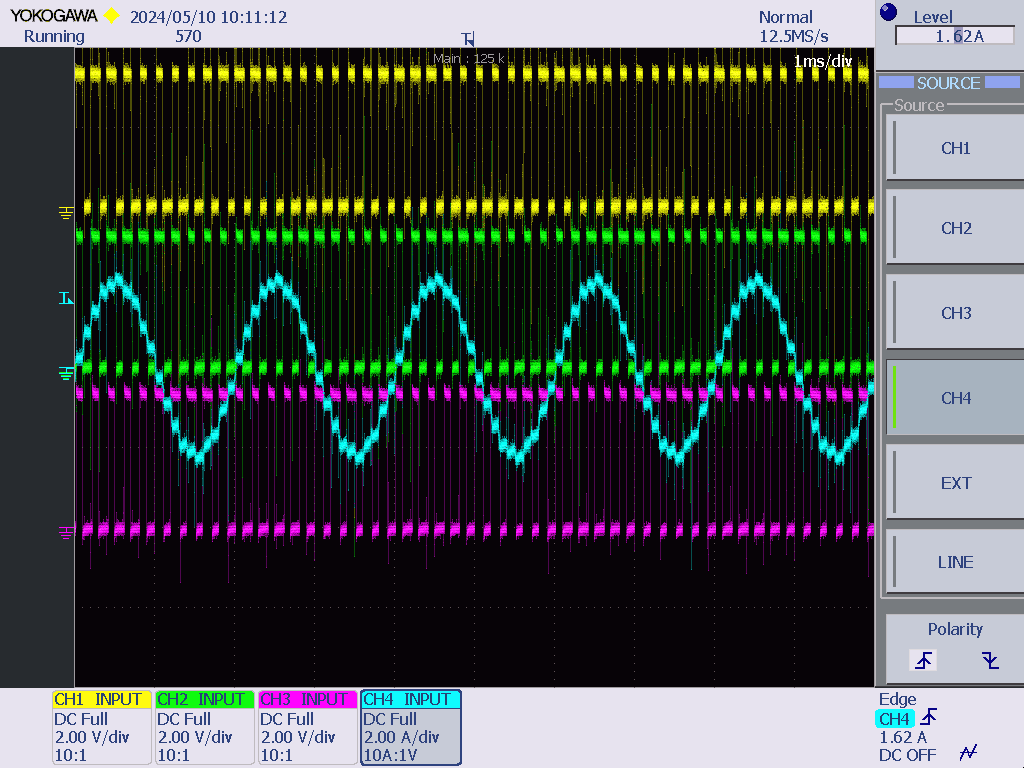
\includegraphics[width=0.7\linewidth]{fig/3RL-PWM}
	\caption{Lazo abierto de tensión. Señales PWM a la entrada del \textit{driver} y corriente de una fase.}
\end{figure}

Se puede validar si la tensión sintetizada es correcta según la corriente de la carga. Se cambió la frecuencia sintetizada a 100 Hz, se ajustó la fuente de tensión a 5 V y se consignó una en el eje $q$ de dos tercios de la máxima disponible, es decir, $(v_d, v_q) = (0, \frac{2}{3}\frac{V_{\text{DC}}}{\sqrt{3}}) = (0, \frac{2}{3}\frac{5 \text{ V,DC}}{\sqrt{3}})$. Se midieron las corrientes de fase para verificar que se estaba modulando correctamente, y se volvió a subir la frecuencia de conmutación para evitar ver el rizado en la carga.

Sabiendo que la tensión en la carga es
\[
v_{\text{fase-neutro, pico}} = i_{\text{fase, pico}}\cdot (R + L\cdot\omega)
\]

y que la tensión modulada es de 

\[ (v_d, v_q) = (0, \frac{2}{3}\frac{5 \text{ V,DC}}{\sqrt{3}}) \text{ V}\]
\[ \therefore v_s = v_q = v_{\text{fase-neutro, pico}} = \frac{2}{3}\frac{5 \text{ V,DC}}{\sqrt{3}} \text{ V ,}\]

se puede calcular que la corriente esperada es de

\[
i_{\text{fase, pico}} = \frac{v_{\text{fase-neutro, pico}}}{(R + L\cdot\omega)} = \frac{\frac{2}{3}\frac{5 \text{ V,DC}}{\sqrt{3}} \text{ V}}{0.8 \text{ }\Omega + 500 \text{\unit{\micro\henry}} \cdot 2\pi100 \text{ Hz}} = 1.73 \text{ A ,}
\]

que encaja con el valor medido de aproximadamente 1,7 A.


\begin{figure}[H]
	\centering
	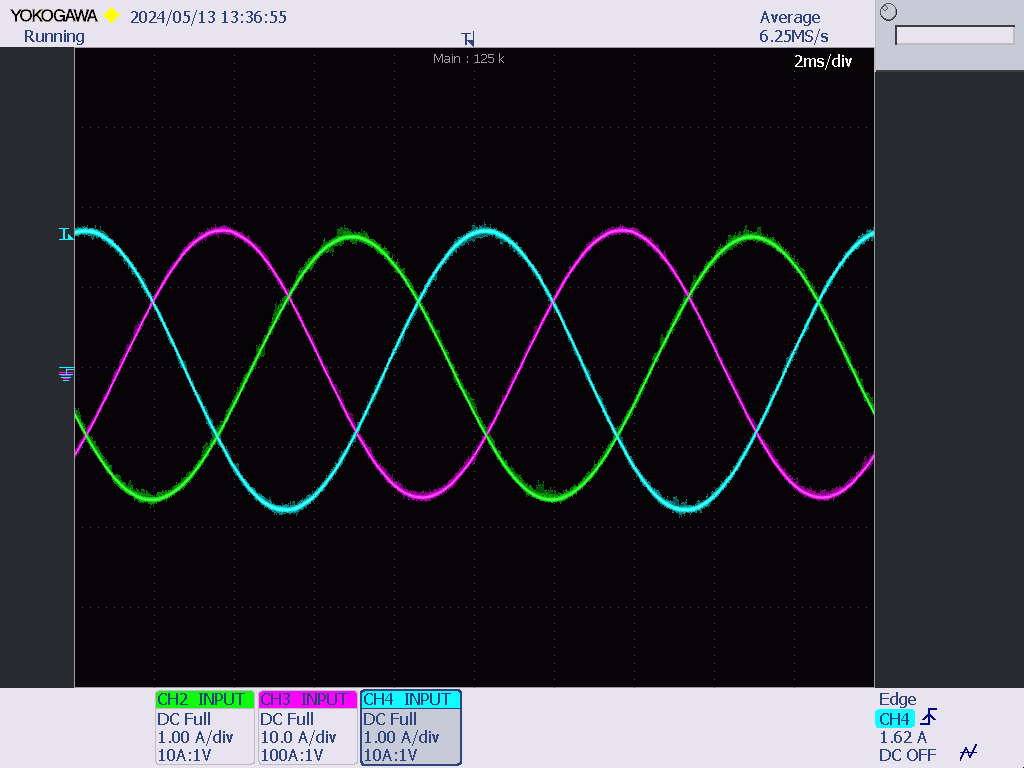
\includegraphics[width=0.7\linewidth]{fig/3RLcurrent}
	\caption{Corrientes de las tres fases de la carga R-L. El canal CH3 muestra un escalado incorrecto, que debería ser igual al de los otros dos canales visibles.}
\end{figure}

\subsection{Lazo abierto de tensión con un PMSM}

Con las tensiones trifásicas correctamente sintetizadas, se probó un lazo abierto de tensión con un PMSM.

\begin{figure}[H]
	\centering
	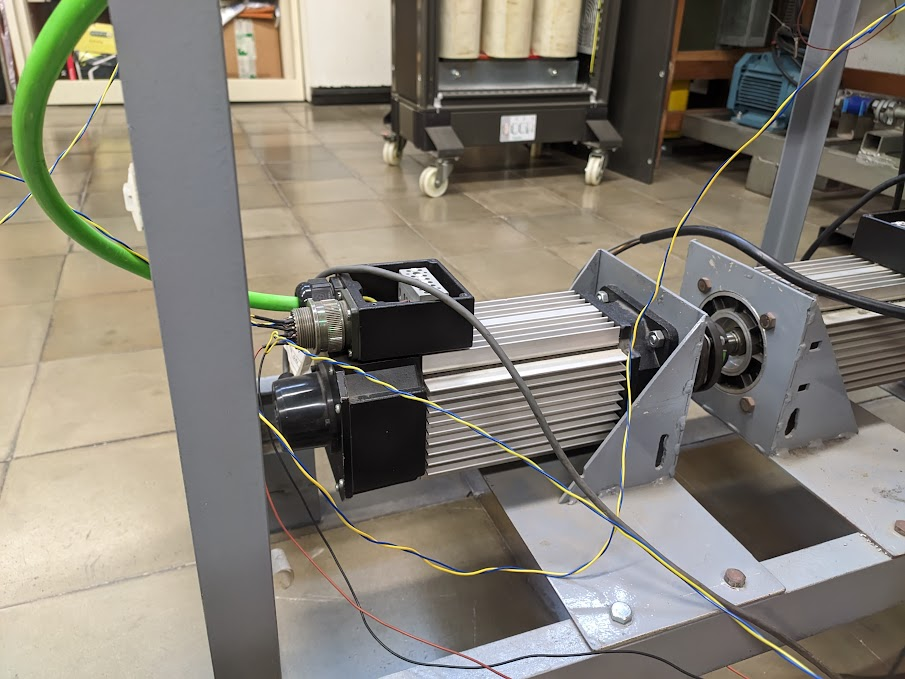
\includegraphics[width=0.7\linewidth]{fig/motorLab}
	\caption{Motor utilizado en los ensayos \cite{mavilor2018}.}
\end{figure}


\begin{table}[H]
	\begin{tabular}{|p{2cm}||r|p{1.5cm}|p{8cm}|}
		\hline
		\multicolumn{4}{|c|}{Parámetros del motor} \\
		\hline
		Parámetro & Valor & Unidades & Descripción \\
		\hline
		\(pp\) & 4 & ad & Número de pares de polos \\
		\(\lambda_m\) & 0,13391 & mWb & Flujo magnético de los imanes permanentes \\
		\(L_d\) & 2,91 & mH & Inductancia en el eje d \\
		\(L_q\) & 2,91 & mH & Inductancia en el eje q \\
		\(R_s\) & 1,95 & \unit{\ohm} & Resistencia de fase del estátor \\
		\(\omega_{\text{m,máx}}\) & 8500 & RPM & Velocidad angular máxima del motor \\
		\(T_{\text{em,máx}}\) & 10 & \unit{N \cdot m} & Par máximo del motor \\
		\(V_{\text{DC,máx}}\) & 450 & \unit{V} & Voltaje máximo DC \\
		\(I_{\text{s,máx}}\) & 60 & \unit{A} & Corriente máxima en los ejes d-q \\
		\hline
	\end{tabular}
	\caption{Parámetros del motor utilizado en los ensayos.}
\end{table}

\begin{figure}[H]
	\centering
	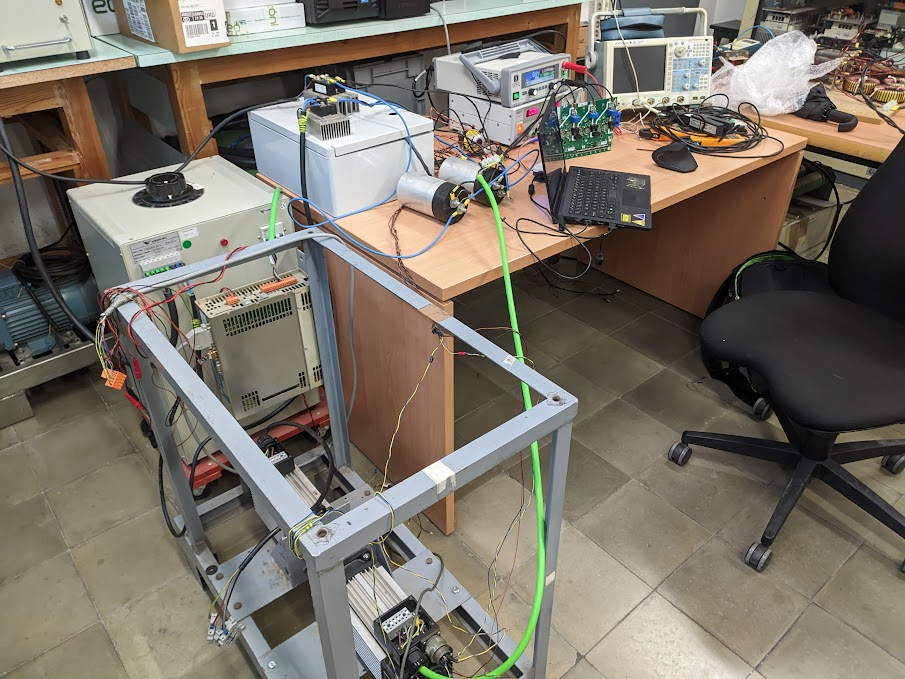
\includegraphics[width=0.7\linewidth]{fig/Mavilor-setup}
	\caption{\textit{Setup} del ensayo con el motor.}
\end{figure}

Se procedió de manera muy similar al ensayo de la carga estática, aunque en este caso fue necesario implementar una rampa de frecuencia para lograr que el motor girara. El resto fue idéntico, y se tomó una captura de las corrientes de fase.


\begin{figure}[H]
	\centering
	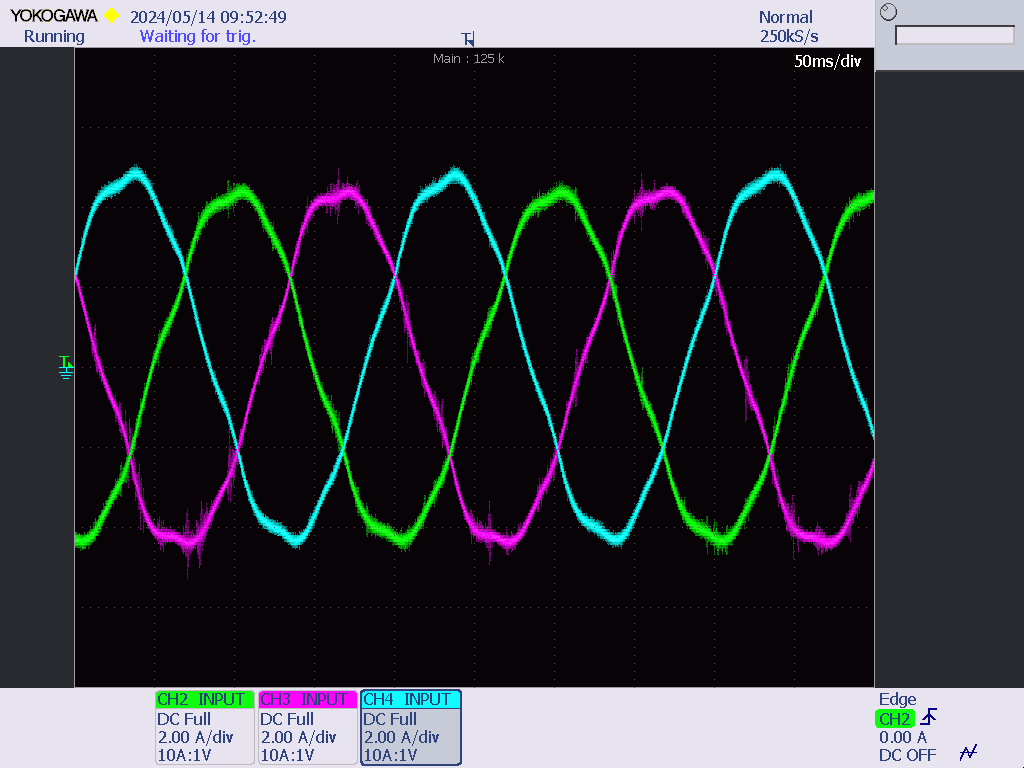
\includegraphics[width=0.7\linewidth]{fig/mavilorCurrent}
	\caption{Corrientes de fase del motor.}
\end{figure}

Como se puede observar, las formas de onda no son perfectamente senoidales, y este hecho se asocia a los armónicos que pueda presentar el bobinado del estátor. La frecuencia sintetizada fue de tan solo 5 Hz, atendiendo a un análisis de estabilidad \cite{Montesinos2008}.


